\chapter{Chiral deformation quantization}
\label{ch:chiral-deformation}
\label{chap:chiral-deformation}
% Regime III: filtered-complete (Convention~\ref{conv:regime-tags}).

\index{deformation quantization!chiral|textbf}

A coisson algebra on a curve~$X$ is a commutative $\cD_X$-algebra with
a Lie$^*$ bracket. After choosing a formal coordinate on a disk it is
seen as a Poisson vertex algebra; without that coordinate it remains a
Beilinson--Drinfeld object. A deformation quantization is a filtered
chiral algebra $\cA_\hbar$ with
$\operatorname{gr}_\hbar \cA_\hbar \simeq \cA_{\mathrm{cl}}$ and whose
first commutator recovers the Lie$^*$ bracket. Existence is a
Maurer--Cartan lifting problem in the completed chiral deformation
complex. Kontsevich--Tamarkin formality supplies the local disk input;
descent along~$X$ and the modular obstruction classes are additional
conditions, not consequences of the local theorem.

The chiral quantization problem has three structural features absent
from the classical Kontsevich theory:
\begin{enumerate}[label=\textup{(\roman*)}]
\item \emph{Curvature.} In the modular regime of this volume, the
 scalar projection of the non-separating genus contribution is
 $\kappa(\cA)\lambda_g$ (Theorem~D). This is a statement about the
 modular Maurer--Cartan element, not a universal assertion that every
 local star product becomes a curved $\Ainf$-algebra on every curve.
\item \emph{Filtration.} The star product is a formal power series
 in~$\hbar$; the $\hbar$-adic filtration corresponds to the weight
 filtration on~$\gAmod$.
\item \emph{Higher obstructions.} The obstruction to extending a
 quantization from order~$\hbar^n$ to~$\hbar^{n+1}$ is the degree-$2$
 class in the controlling shifted dg Lie algebra; in unshifted
 Hochschild conventions this is the familiar degree-$3$ obstruction.
 The qualifier ``chiral'' is mandatory: the complex is
 $\ChirHoch^\bullet(\cA,\cA)$, not categorical or topological
 Hochschild cohomology (Convention~\ref{conv:three-hochschild}).
\end{enumerate}
Kontsevich's formula and the chiral bar differential share the same
local combinatorics: Fulton--MacPherson boundary strata, logarithmic
collision classes, and Arnold relations. The forms are not literally
the same. Kontsevich integrates angle forms on compactified
configurations in the upper half-plane; the chiral bar construction
uses residue classes such as $\eta_{ij}=d\log(z_i-z_j)$ on
configurations of points on~$X$. The bridge is a local comparison of
boundary-factorisation identities, followed by a separate global
descent problem.

\section{Kontsevich's theorem}

\begin{theorem}[Kontsevich 1997 \cite{Kon03}; \ClaimStatusProvedElsewhere]
\label{thm:kontsevich-star-product}
Let $(M,\pi)$ be a Poisson manifold with Poisson bivector
$\pi\in\Gamma(\wedge^2TM)$. There exists a star product
\[
\star\colon C^\infty(M)[[\hbar]]\otimes C^\infty(M)[[\hbar]]
\longrightarrow C^\infty(M)[[\hbar]]
\]
such that:
\begin{enumerate}
\item $f \star g = fg + \frac{\hbar}{2}\{f,g\} + O(\hbar^2)$
\item $(f \star g) \star h - f \star (g \star h) = 0$ (associativity)
\item The star product is given by an explicit formula:
\[
f\star g
=fg+\sum_{n\geq1}\hbar^n
\sum_{\Gamma\in\mathcal G_{n,2}}
\frac{w_\Gamma}{|\operatorname{Aut}(\Gamma)|}\,B_\Gamma(f,g).
\]
Here $\mathcal G_{n,2}$ is the set of admissible directed graphs with
$n$ internal vertices and two boundary vertices, $B_\Gamma$ is the
bidifferential operator determined by the directed edges and the
Poisson tensor, and \(w_\Gamma\) is the angle-form integral over
\(\overline C_{n,2}(\mathbb H)\).
\end{enumerate}
\end{theorem}

\subsection{The configuration space construction}

The configuration spaces here are the upper-half-plane analogues of the
collision spaces used by the Heisenberg bar differential
(\S\ref{sec:frame-bar-deg2}). They are not identical spaces: the
Kontsevich construction has two ordered boundary insertions and
internal points in \(\mathbb H\).

The weight \(w_\Gamma\) for a graph \(\Gamma\in\mathcal G_{n,2}\) is:
\[
w_\Gamma
=\frac{1}{(2\pi)^{2n}}
\int_{\overline C_{n,2}(\mathbb H)}\omega_\Gamma
\]
where (see Cattaneo--Felder \cite{CattaneoFelder99} for the path integral interpretation):
\begin{itemize}
\item $\overline C_{n,2}(\mathbb H)$ is Kontsevich's compactified
configuration space of \(n\) labelled internal points in the upper
half-plane and two ordered boundary points, modulo real translations
and positive dilations;
\item $\omega_\Gamma$ is a differential form constructed from the graph $\Gamma$:
\[\omega_\Gamma = \bigwedge_{e \in E(\Gamma)} d\phi_e\]
where $\phi_e = \arg(z_{\text{target}(e)} - z_{\text{source}(e)})$ is the angle of edge $e$
\end{itemize}

\begin{example}[The first quantum correction]
At order $\hbar$, the unique admissible graph has one internal vertex in $\mathbb{H}$ with edges to the two boundary points $f, g$ on $\mathbb{R}$:
\begin{center}
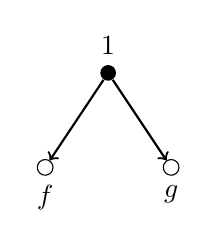
\begin{tikzpicture}[scale=0.8]
\node[circle,fill,inner sep=2pt,label=above:{$1$}] (1) at (1,1.5) {};
\node[circle,draw,inner sep=2pt,label=below:{$f$}] (f) at (0,0) {};
\node[circle,draw,inner sep=2pt,label=below:{$g$}] (g) at (2,0) {};
\draw[->,thick] (1) -- (f);
\draw[->,thick] (1) -- (g);
\end{tikzpicture}
\end{center}

The Kontsevich weight is:
\[w_\Gamma = \frac{1}{(2\pi)^2}\int_{\mathbb{H}} d\phi_{1f} \wedge d\phi_{1g} = \frac{1}{2}\]
where $\phi_{1f} = \arg(f - z_1)$ and $\phi_{1g} = \arg(g - z_1)$ are the angles from the internal vertex $z_1 \in \mathbb{H}$ to the boundary points. The bidifferential operator is $B_\Gamma(f,g) = \pi^{ij}\partial_i f \cdot \partial_j g = \{f, g\}$, giving:
\[f \star g = fg + \frac{\hbar}{2}\{f,g\} + O(\hbar^2)\]
\end{example}

\subsection{Role of the upper half-plane}

The upper half-plane $\mathbb{H}$ is the basic bordered surface in
Kontsevich's construction: boundary insertions lie on
\(\mathbb R\subset\partial\mathbb H\), internal vertices lie in
\(\mathbb H\), and the normalization quotients by the affine group of
the real line. The compactifications
\(\overline C_{n,m}(\mathbb H)\) have Fulton--MacPherson boundary
strata governed by the Stasheff associahedra and the little-disks
operad. This is the source of the Stokes identities in the star-product
proof.

\section{Chiral algebras as quantum observables}

\subsection{From Poisson to chiral}

Replacing the Poisson manifold with a curve \(X\), the analogue of a
Poisson structure is a \emph{coisson structure} in the sense of
Beilinson--Drinfeld. After choosing a formal coordinate, the same local
datum is written as a Poisson vertex algebra structure.

\begin{remark}[Coisson algebra on a curve; cf.\ Definition~\ref{def:coisson}]
\label{rem:coisson-curve}
A \emph{coisson algebra} on a smooth curve $X$ is a sheaf
$\mathcal{A}$ of commutative $\mathcal{D}_X$-algebras with a
Lie$^*$ bracket. After choosing a coordinate on a formal disk this
bracket is written as a Poisson vertex algebra $\lambda$-bracket:
\[\{a(z), b(w)\} = \sum_{k=1}^N \frac{P_k(a,b)(w)}{(z-w)^k}\]
where $P_k$ are bidifferential operators, satisfying Jacobi and Leibniz.
A coisson algebra is \emph{not} a chiral algebra: it is a commutative
$\mathcal{D}$-module with bracket data encoding the singular part of a
potential OPE. A filtered quantization, when it exists, is a chiral
algebra whose associated graded is the coisson algebra. In vertex
language this is an $\Einf$-chiral algebra; ordered Yangian and RTT
data live in the $\Eone$ layer and are not supplied by the PVA bracket
alone. For the gauge-theoretic origin of PVA structures via 3d
holomorphic-topological theories, see Khan--Zeng~\cite{KhanZeng25}
(scope: freely generated PVA with conformal vector at non-critical
level).
\end{remark}

\begin{construction}[Deformation quantization as shadow-level MC]
\label{constr:dq-shadow-mc}
\index{deformation quantization!shadow MC}
Let $V^{\mathrm{cl}}$ be the local PVA attached to a coisson algebra
after choosing a coordinate. The deformation-quantization problem is
the problem of lifting the classical bracket to an $\hbar$-adic
Maurer--Cartan element:
\begin{enumerate}[label=\textup{(\roman*)}]
\item The classical limit carries a Poisson $\lambda$-bracket
 $\{a_\lambda b\}$; in the modular notation it is the degree-$2$ local
 shadow of the ordered Maurer--Cartan element.
\item The PVA Jacobi identity says precisely that this degree-$2$
 piece solves the Maurer--Cartan equation modulo $\hbar^2$.
\item The next obstruction is the degree-$2$ cohomology class in the
 shifted chiral deformation dg Lie algebra (degree~$3$ in unshifted
 Hochschild notation). Higher obstructions $o_r$ for $r \geq 4$ are
 governed by the shadow obstruction tower of the candidate quantized
 algebra and do not automatically vanish. Koszulness of the quantized
 algebra is separate from shadow obstruction tower termination; both
 finite and infinite shadow-depth algebras can be Koszul.
\end{enumerate}
\end{construction}

\begin{example}[Current algebra]
For a Lie algebra $\mathfrak g$, the unextended current PVA has
\[
\{J^a(z),J^b(w)\}=\frac{f^{ab}_{\phantom{ab}c}J^c(w)}{z-w}.
\]
Choosing an invariant bilinear form \(B\) adds the central PVA term
\[
\{J^a_\lambda J^b\}=f^{ab}_{\phantom{ab}c}J^c+B(J^a,J^b)\lambda .
\]
The affine vertex algebra \(V_k(\mathfrak g)\) is the filtered
quantization of this centrally extended current PVA with
\(B=k(\cdot,\cdot)\). The level is an input pairing, not the limit
\(k\to\infty\).
\end{example}

\subsection{Operator product expansion as filtered product}

The singular OPE of a filtered chiral quantization is the chiral
analogue of a star product:
\[a(z) \cdot b(w) = \sum_{k=0}^\infty \frac{(a *_k b)(w)}{(z-w)^k}\]

This has the same structure as Kontsevich's formula: the classical term is $a(z)b(w)$ (commutative product), the first quantum correction is $\frac{\{a, b\}(w)}{z-w}$ (Poisson bracket), and the higher quantum corrections are $\frac{(a *_k b)(w)}{(z-w)^k}$.

\begin{convention}[Independent parameters in deformation quantization]
\label{conv:defq-parameter-separation}
\index{deformation quantization!parameter separation}
Five parameters occur in this chapter, and they live in different
objects.
\begin{enumerate}[label=\textup{(\roman*)}]
\item The affine level \(k\) is the scalar multiplying the invariant
 bilinear form in the central extension of a current algebra.
\item The KZ coefficient is the separate rational factor
 \((k+h^\vee)^{-1}\) in the Knizhnik--Zamolodchikov connection
 \[
 \nabla_i^{\mathrm{KZ}}
 =\partial_{z_i}
 +\sum_{j\ne i}\frac{\Omega_{ij}}{(k+h^\vee)(z_i-z_j)}
 \qquad\textup{\cite{KZ84,Kohno87}}.
 \]
 It is not the affine level.
\item The Yangian/RTT spectral parameter \(u\) is the meromorphic
 loop/evaluation coordinate in tensors such as \(R(u)\) and \(r(u)\).
 It is not the KZ coefficient.
\item The formal deformation parameter \(\hbar\) is the filtration
 variable in star products, \(R=1+\hbar r+O(\hbar^2)\), and
 \(\Def_{\mathrm{ch}}(-)[[\hbar]]\). It is not a period, a level, or
 a spectral parameter.
\item The genus-counting or string coupling variable, denoted
 \(q_{\mathrm{gen}}\) in the modular MC expansion and \(g_s\) in a
 physical partition function, records stable-graph genus. Identifying
 it with \(\hbar\) requires a chosen quantum field theory and a
 normalization theorem.
\end{enumerate}
\end{convention}

\begin{theorem}[Local coisson quantization and global obstruction; \ClaimStatusProvedHere]\label{thm:chiral-quantization}
Let $\cA_{\mathrm{cl}}$ be a coisson algebra on a smooth curve~$X$.
Filtered chiral quantizations of $\cA_{\mathrm{cl}}$ with fixed
associated graded are classified, when the usual pronilpotence and
completeness hypotheses hold, by gauge classes of Maurer--Cartan lifts
of the Lie$^*$ bracket in the completed chiral deformation dg Lie
algebra
\[
\Def_{\mathrm{ch}}(\cA_{\mathrm{cl}})[[\hbar]].
\]
On a formal disk, for a finite-type local PVA coming from a formal
Poisson structure, Kontsevich--Tamarkin formality supplies such a lift.
On a curve~$X$, the local lifts glue to a global chiral quantization
if and only if the descent class and the modular obstruction classes
in the same completed deformation complex vanish.
\end{theorem}

\begin{remark}[Higher genus extension]\label{rem:chiral-quantization-higher-genus}
The higher-genus extension is a modular deformation problem, not a
formal consequence of genus-$0$ Kontsevich formality. It requires
control of the non-separating clutching term and the stable-graph
boundary relations on $\overline{\mathcal{M}}_{g,n}$.
\end{remark}

\begin{proof}[Proof of Theorem~\ref{thm:chiral-quantization}]
The completed chiral deformation complex carries the usual dg Lie
structure: the differential is the linearized chiral product and the
bracket is insertion of operations. The standard Deligne--Hinich
argument identifies gauge classes of Maurer--Cartan elements in a
pronilpotent dg Lie algebra with filtered deformations of the
underlying algebraic structure. In the present notation the first
coefficient of the Maurer--Cartan element is the Lie$^*$ bracket on
$\cA_{\mathrm{cl}}$.

On a formal disk the coordinate identifies the coisson algebra with a
PVA, and for finite-type formal Poisson input the
Kontsevich--Tamarkin formality quasi-isomorphism transfers the Poisson
Maurer--Cartan element to an associative $\hbar$-adic product. The
geometric--operadic bar comparison
(Theorem~\ref{thm:geometric-equals-operadic-bar}) identifies the local
bar differential with the chiral deformation complex on the disk; it
does not by itself perform global descent. Gluing the local
Maurer--Cartan elements across~$X$ is exactly the vanishing of the
descent and modular obstruction classes in
\(\Def_{\mathrm{ch}}(\cA_{\mathrm{cl}})[[\hbar]]\).
\end{proof}

\section{Configuration space integrals for chiral algebras}

\subsection{The local comparison space}

Kontsevich's configuration space is not replaced by a single global
``chiral configuration space''. The comparison is local on the formal
disk and global only after descent.

\begin{definition}[Local chiral configuration model]
Fix a formal coordinate on a disk $D\subset X$. The local comparison
space is the Fulton--MacPherson compactification
\[
\overline{\Conf}_n(D)
\]
with collision divisors labelled by rooted trees. Its residue forms are
generated by
\[
\eta_{ij}=d\log(z_i-z_j),
\]
and its boundary strata encode the partial compositions in the chiral
bar construction. A change of coordinate acts on this model by the
Aut$(\mathcal O)$-torsor of formal coordinates; descending from the
disk to~$X$ is a separate equivariance condition.
\end{definition}

\subsection{Forms on chiral configuration spaces}

The local chiral bar complex uses \emph{logarithmic forms with
coefficients}; integration appears only after a propagator and a
cycle/top-dimensional chain have been specified.

\begin{definition}[Chiral residue forms]
On $\overline{\Conf}_n(D)$, the local chiral bar forms are
\[
\Omega^*_{\mathrm{ch,loc}}
= \Omega^*_{\log}(\overline{\Conf}_n(D))\otimes\mathcal{A}^{\boxtimes n}
\]
where:
\begin{itemize}
\item $\Omega^*_{\text{log}}$ are logarithmic forms with poles along collision divisors:
\[\eta_{ij} = d\log(z_i - z_j) = \frac{dz_i - dz_j}{z_i - z_j}\]
\item $\mathcal{A}^{\boxtimes n} = \mathcal{A}|_{z_1} \boxtimes \cdots \boxtimes \mathcal{A}|_{z_n}$ are field insertions
\end{itemize}
\end{definition}

\subsection{The chiral star product formula}

\begin{theorem}[Local Kontsevich--chiral comparison; \ClaimStatusProvedHere]
\label{thm:chiral-kontsevich}
\index{star product}
Let $\mathcal{A}_{\mathrm{cl}}$ be a coisson algebra on~$X$, and fix a
formal disk $D\subset X$ on which its restriction is a finite-type PVA
coming from a formal Poisson structure. The local Kontsevich product is
\[
a\star b
=ab+\sum_{n\geq1}\hbar^n
\sum_{\Gamma\in\mathcal G_{n,2}}
\frac{w_\Gamma}{|\operatorname{Aut}(\Gamma)|}\,B_\Gamma(a,b),
\]
where:
\begin{enumerate}
\item $\mathcal{G}_{n,2}$ is Kontsevich's set of admissible graphs
 with $n$ internal and two boundary vertices;
\item $B_\Gamma(a,b)$ is the bidifferential operator determined by the
 Poisson tensor and the directed edges of~$\Gamma$;
\item $w_\Gamma$ is the upper-half-plane angle-form integral on
 $\overline{C}_{n,2}(\mathbb H)$.
\end{enumerate}
Under Theorem~\ref{thm:geometric-equals-operadic-bar}, the boundary
factorisation identities for these local weights map to the quadratic
identities of the chiral bar differential on~$D$. This comparison does
not assert a global formula
\(\int_{\overline{C}_n(X)}B_\Gamma\wedge\omega_\Gamma\) for an
arbitrary curve~$X$; global quantization still requires coordinate
descent and vanishing modular obstructions.
\end{theorem}

\begin{proof}
Kontsevich's theorem gives the displayed product on the formal disk by
integrating angle forms over $\overline{C}_{n,2}(\mathbb H)$. Its
associativity is the Stokes identity on the compactified
upper-half-plane configuration spaces, together with the vanishing
lemma for the angle forms.

The chiral bar differential on a disk is computed by the same rooted
collision trees. The form attached to an edge is now represented by the
residue class $\eta_{ij}=d\log(z_i-z_j)$, and the Arnold relation is the
quadratic identity forcing $d_B^2=0$. The
geometric--operadic comparison identifies these two boundary
factorisation systems after passing from the local disk to the
operadic bar construction. This proves the local comparison. A global
curve has coordinate-change and modular boundary terms; those are
precisely the descent and obstruction classes named in
Theorem~\ref{thm:chiral-quantization}.
\end{proof}

\begin{remark}[Provenance]
The analytic integral formula is Kontsevich's upper-half-plane formula
\cite{Kon03}. The chiral statement used here is the local comparison
between Kontsevich boundary strata and the geometric bar construction,
not a new closed-form global star product on
$\overline{\Conf}_n(X)$.
\end{remark}

\section{Explicit computations through degree 5}

\subsection{Organization by loop order}

The low-order coefficients fix the normalization.

\subsubsection{\texorpdfstring{Tree level ($\hbar^0$): classical product}{Tree level (0): classical product}}

\[a \star_0 b = ab\]

Graph: Just two vertices, no edges.

\subsubsection{\texorpdfstring{One loop ($\hbar^1$): Poisson bracket}{One loop (1): Poisson bracket}}

\[a \star_1 b = \frac{1}{2}\{a, b\}\]

Graph: One interior vertex in $\mathbb{H}$ with two directed edges to the two boundary vertices (representing $a$ and $b$).

Weight calculation:
\[
w_\Gamma
=\frac{1}{(2\pi)^2}
\int_{\overline C_{1,2}(\mathbb H)}
d\phi_{1f}\wedge d\phi_{1g}
=\frac12 .
\]
This is Kontsevich's upper-half-plane integral. The local chiral
residue form \(\eta_{ij}=d\log(z_i-z_j)\) is compared with it only
after choosing a formal disk and passing to boundary-factorisation
identities; no integral over a global
\(C_2^{\mathrm{ch}}(X)\) is used in this coefficient.

\subsubsection{\texorpdfstring{Two loops ($\hbar^2$): first quantum correction}{Two loops (2): first quantum correction}}

There are three operator types contributing at $\hbar^2$:

\emph{Graph~1.} Two independent Poisson vertices, each with one edge
to the \(a\)-boundary vertex and one edge to the \(b\)-boundary
vertex; there is no internal edge.

\[B_{\Gamma_1}(a,b) = \pi^{ij} \pi^{kl} \frac{\partial^2 a}{\partial x^i \partial x^k} \frac{\partial^2 b}{\partial x^j \partial x^l}\]

Weight: \(w_{\Gamma_1}=\frac18\), in the normalization where the
first-order coefficient is \(\frac12\{a,b\}\), computed by the
Kontsevich integral on \(\overline C_{2,2}(\mathfrak H)\).

\emph{Graph~2.} One internal edge differentiates the second Poisson
tensor, and the remaining boundary edges land on \(a\) and \(b\) in
the order displayed below.

\[B_{\Gamma_2}(a,b) = \pi^{ij} (\partial_j\pi^{kl})\, \partial_i\partial_k a \cdot \partial_l b\]

Weight: \(w_{\Gamma_2}=\frac1{12}\) in the same normalization.

\emph{Graph~3.} Same topology as Graph 2 with $a \leftrightarrow b$

\[B_{\Gamma_3}(a,b) = \pi^{ij} (\partial_j\pi^{kl})\, \partial_k a \cdot \partial_i\partial_l b\]

Weight: \(w_{\Gamma_3}=\frac1{12}\). The sign in
\(B_{\Gamma_2}-B_{\Gamma_3}\) is the bidifferential-operator sign
from the Poisson tensor convention, not a claim about a global chiral
orientation integral.

\emph{Total at $\hbar^2$.}
\[a \star_2 b = \frac{1}{8}B_{\Gamma_1}(a,b) + \frac{1}{12}\bigl(B_{\Gamma_2} - B_{\Gamma_3}\bigr)(a,b)\]

This matches the standard Kontsevich formula: the $1/8$ coefficient for the double-Poisson graph and $1/12$ for the $\partial\pi$ graphs (cf.\ the explicit second-order computation below).

\begin{theorem}[Explicit formula \cite{Kon03}; \ClaimStatusProvedElsewhere]
\label{thm:kontsevich-explicit-formula}
\[a \star b = ab + \frac{\hbar}{2}\{a,b\} + \hbar^2\!\left(\frac{1}{8}\pi^{ij}\pi^{kl}\partial_i\partial_k a\,\partial_j\partial_l b + \frac{1}{12}\pi^{ij}(\partial_j\pi^{kl})(\partial_i\partial_k a\,\partial_l b - \partial_k a\,\partial_i\partial_l b)\right) + O(\hbar^3)\]
\end{theorem}

\subsection{\texorpdfstring{Order $\hbar^3$: Stokes cancellation}{Order 3: Stokes cancellation}}

At order $\hbar^3$ the star product is already required to be
strictly associative:
\[
(a\star b)\star c-a\star(b\star c)=0.
\]
The relevant cancellation is a Stokes identity on
\(\overline C_{3,2}(\mathbb H)\). It is not the Drinfeld associator of
the KZ equation; that associator enters when one compares formality
representatives and braided tensor structures.

\begin{theorem}[Stokes' theorem yields associativity \cite{Kon03};
\ClaimStatusProvedElsewhere]
\label{thm:stokes-associativity}
\[
\sum_{\Gamma\in\mathcal G_{3,2}^{\mathrm{adm}}}
\epsilon_\Gamma w_\Gamma\,
(\text{boundary graph operation})=0
\]
because:
\[\int_{\partial \overline{C}_{3,2}(\mathbb H)} \omega = 0\]
by Stokes' theorem.
\end{theorem}

\emph{Stasheff pentagon.}
The codimension-one boundary strata form the pentagon \(K_4\):
\begin{center}
\begin{tikzpicture}[scale=1.2]
\node (a) at (90:1.5) {$\Gamma_1$};
\node (b) at (162:1.5) {$\Gamma_2$};
\node (c) at (234:1.5) {$\Gamma_3$};
\node (d) at (306:1.5) {$\Gamma_4$};
\node (e) at (18:1.5) {$\Gamma_5$};
\draw[->] (a) -- (b);
\draw[->] (b) -- (c);
\draw[->] (c) -- (d);
\draw[->] (d) -- (e);
\draw[->] (e) -- (a);
\end{tikzpicture}
\end{center}
This pentagon is the associahedral boundary relation for four inputs.
Calling it the KZ/Drinfeld associator conflates the Stasheff
boundary cell with the monodromy associator of the KZ connection.

\subsection{Four and five loops}

\subsubsection{\texorpdfstring{Four loops ($\hbar^4$)}{Four loops (4)}}

At $\hbar^4$, Kontsevich admissible graphs on the upper half-plane
produce period integrals. For associator choices coming from the KZ
connection, the first odd zeta value $\zeta(3)$ appears in the
corresponding Drinfeld associator coefficients. No equality
\(\int_{\overline{C}_4(X)}\omega=\zeta(3)/(2\pi i)^3\) is used here:
that is a global curve integral, not the local
upper-half-plane weight.

\subsubsection{\texorpdfstring{Five loops ($\hbar^5$)}{Five loops (5)}}

At $\hbar^5$, the same period mechanism produces higher associator
coefficients. Depending on the chosen associator representative,
multiple zeta values such as $\zeta(3)$ and $\zeta(5)$ occur. The
precise graph count and the individual weights are not part of the
chiral bar argument in this chapter.

\begin{example}[Explicit weight at \texorpdfstring{$\hbar^5$}{5}]
For the KZ associator, the depth-one coefficient attached to the
degree-$5$ Lie word is proportional to $\zeta(5)/(2\pi i)^5$.
Identifying a specific Kontsevich graph weight with that coefficient
requires fixing the graph representative and the associator gauge.
\end{example}

\section{Bar-cobar realization of deformation quantization}

\subsection{Bar complex and deformation}

\begin{theorem}[Chiral deformation complex from the bar construction; \ClaimStatusProvedHere]
\label{thm:bar-computes-deformation}
Let $\mathcal A_{\mathrm{cl}}$ be a coisson algebra satisfying the
completion hypotheses of Theorem~\ref{thm:chiral-quantization}. The
reduced geometric bar construction realizes a strict model for the
shifted chiral deformation dg Lie algebra:
\[
\Def_{\mathrm{ch}}(\mathcal A_{\mathrm{cl}})
\simeq
\operatorname{Coder}\bigl(\barBgeom(\mathcal A_{\mathrm{cl}})\bigr)[1].
\]
Consequently filtered quantizations are Maurer--Cartan elements modulo
gauge, not the cohomology group itself. The cohomology groups measure
the successive tangent and obstruction spaces:
\begin{enumerate}
\item $H^0$ of the shifted dg Lie algebra: infinitesimal stabilizers;
\item $H^1$: first-order deformations modulo infinitesimal gauge;
\item $H^2$: obstruction classes in the shifted convention;
\item equivalently, in unshifted chiral Hochschild notation, first
 order deformations lie in $\ChirHoch^2$ and primary obstructions in
 $\ChirHoch^3$.
\end{enumerate}
\end{theorem}

\begin{remark}[Object firewall for deformation quantization]
\label{rem:defq-object-firewall}
The deformation complex above separates five objects.
\[
A,\qquad \barB(A),\qquad A^{\mathrm i},\qquad A^!,\qquad
Z^{\mathrm{der}}_{\mathrm{ch}}(A).
\]
Here \(A=\mathcal A_{\mathrm{cl}}\) is the coisson input,
\(\barB(A)\) is the reduced bar coalgebra whose coderivations form the
shifted deformation dg Lie algebra, \(A^{\mathrm i}=H^\bullet\barB(A)\)
is the Koszul dual coalgebra when the Koszul hypotheses hold, and
\(A^!=\mathbb D(A^{\mathrm i})\) is the Verdier-dual Koszul dual
algebra. The derived chiral centre
\[
Z^{\mathrm{der}}_{\mathrm{ch}}(A)
\simeq C^\bullet_{\mathrm{ch}}(A,A)
\]
is the Hochschild closed-sector object. Maurer--Cartan quantization lives in
coderivations of \(\barB(A)\); it is not an element of \(A^!\) and not
an element of the derived centre. The equality
\(\Omega(\barB(A))\simeq A\), when it holds, is bar--cobar inversion,
not Koszul duality.
\end{remark}

\subsection{Maurer--Cartan elements as quantizations}

The quantization is a solution to the Maurer--Cartan equation in the
completed shifted chiral deformation object. In a strict dg Lie model
this equation is
\[
d\alpha+\frac12[\alpha,\alpha]=0.
\]
After homotopy transfer to a minimal \(L_\infty\)-model it becomes
\[
\sum_{r\geq1}\frac1{r!}\ell_r(\alpha,\ldots,\alpha)=0,
\]
where \(\ell_1=d\), \(\ell_2=[-,-]\), and the higher brackets record
the transferred bar operations.

\begin{proposition}[MC elements and filtered chiral products; \ClaimStatusProvedHere]
\label{prop:mc-star-product}
Gauge classes of Maurer--Cartan elements
\(\alpha\in\Def_{\mathrm{ch}}(\mathcal{A}_{\mathrm{cl}})^1[[\hbar]]\)
in any complete \(L_\infty\)-model for the chiral deformation functor
whose linear term is the prescribed Lie$^*$ bracket are in bijection
with filtered chiral products on $\mathcal{A}_{\mathrm{cl}}[[\hbar]]$
whose associated graded product is the commutative product on
$\mathcal{A}_{\mathrm{cl}}$.
\end{proposition}

\begin{proof}
Given an MC element
$\alpha=\sum_{n\geq1}\hbar^n\alpha_n$, insert the multilinear
operation $\alpha_n$ as the $\hbar^n$ correction to the chiral product.
The MC equation unfolds order by order:
\[
d\alpha_n+\frac12\sum_{i+j=n}[\alpha_i,\alpha_j]
+\sum_{r\geq3}\frac1{r!}
\sum_{i_1+\cdots+i_r=n}
\ell_r(\alpha_{i_1},\ldots,\alpha_{i_r})=0.
\]
This is exactly the $n$-th filtered associativity/factorisation
identity, because $d$ is the linearized bar differential and the
brackets are insertion of lower-order operations. Gauge equivalence is
the Deligne--Getzler equivalence relation for the complete
\(L_\infty\)-algebra; in a strict dg Lie representative it is the usual
degree-$0$ conjugation. The converse reads the coefficients of any such
product as the components of an MC element.
\end{proof}

\begin{lemma}[Shifted obstruction cocycle]
\label{lem:defq-shifted-obstruction-cocycle}
\ClaimStatusProvedHere
Let
\[
\alpha_{<N}=\sum_{1\leq n<N}\hbar^n\alpha_n
\in
\Def_{\mathrm{ch}}(\mathcal A_{\mathrm{cl}})^1[[\hbar]]/(\hbar^N)
\]
solve the \(L_\infty\) Maurer--Cartan equation modulo \(\hbar^N\).
The obstruction to extending it through order~\(\hbar^N\) is the
degree-\(2\) cocycle
\begin{equation}\label{eq:defq-obstruction-cocycle}
\operatorname{Obs}_N(\alpha_{<N})
=
\frac12\sum_{\substack{i+j=N\\ i,j\geq1}}
[\alpha_i,\alpha_j]
+
\sum_{r\geq3}\frac1{r!}
\sum_{\substack{i_1+\cdots+i_r=N\\ i_j\geq1}}
\ell_r(\alpha_{i_1},\ldots,\alpha_{i_r}).
\end{equation}
Its class in \(H^2(\Def_{\mathrm{ch}}(\mathcal A_{\mathrm{cl}}))\)
vanishes exactly when one can choose
\(\alpha_N\in\Def_{\mathrm{ch}}(\mathcal A_{\mathrm{cl}})^1\) with
\[
d\alpha_N+\operatorname{Obs}_N(\alpha_{<N})=0.
\]
Thus the Maurer--Cartan element is the filtered product; the
cohomology class records only the obstruction to the next lift.
In unshifted chiral Hochschild notation the same obstruction lies in
\(\ChirHoch^3(\mathcal A_{\mathrm{cl}},\mathcal A_{\mathrm{cl}})\).
\end{lemma}

\begin{proof}
Extract the coefficient of \(\hbar^N\) in
\(\sum_{r\geq1}r!^{-1}\ell_r(\alpha,\ldots,\alpha)=0\), writing
\(\ell_1=d\). The summands involving the unknown coefficient
\(\alpha_N\) occur only in \(d\alpha_N\); every other summand is
\eqref{eq:defq-obstruction-cocycle}. The \(L_\infty\) identities and
the Maurer--Cartan equation modulo \(\hbar^N\) give
\(d\,\operatorname{Obs}_N(\alpha_{<N})=0\). Vanishing of its cohomology
class is precisely the solvability of the displayed inhomogeneous
equation for~\(\alpha_N\).
\end{proof}

\subsection{Configuration spaces as deformation parameters}

The space of quantizations is the Deligne--Getzler Maurer--Cartan
groupoid of the complete deformation \(L_\infty\)-algebra:
\[\mathcal{Q}(\mathcal{A}_{\text{cl}}) =
\MC(\Def_{\mathrm{ch}}(\mathcal{A}_{\text{cl}})[[\hbar]])/\text{gauge}.\]

Geometrically:
\[
\operatorname{gr}\Def_{\mathrm{ch}}(\mathcal{A}_{\text{cl}})
\simeq
\bigoplus_{n\geq2}
\Gamma\bigl(\overline{\Conf}_n(X),
\Omega^\bullet_{\log}\otimes\mathcal A_{\mathrm{cl}}^{\boxtimes n}\bigr)_{\mathrm{res}},
\]
with differential induced by collision residues and the chiral product.

Thus configuration spaces contribute cochains to the deformation
complex. Their closed degree-top forms are not themselves the moduli
space of quantizations.

\section{Examples: quantizing concrete chiral algebras}

\subsection{Example 1: Heisenberg algebra}

\subsubsection{Classical structure}

\[\{a(z), a^*(w)\} = \frac{1}{z-w} \quad \text{(coisson/PVA $\lambda$-bracket)}\]

\subsubsection{Quantization}

The formal family may be written with first correction
\[
a(z)a^*(w)
\sim
\hbar\,\frac{k}{z-w}.
\]
After setting the deformation variable to \(1\), the Heisenberg vertex
algebra has singular OPE
\[
a(z)a^*(w)\sim\frac{k}{z-w}.
\]

The level $k$ is the chosen invariant pairing of the rank-one
Heisenberg system. In the notation of the landscape census the modular
characteristic is $\kappa(\mathcal H_k)=k$; it is not obtained by
integrating a universal one-form over the curve.

\subsubsection{Configuration space formula}

Locally on a disk, the residue of the propagator is normalized by
\[
\operatorname{Res}_{z=w}\eta_{12}=1.
\]
The coefficient multiplying this residue is the external level~$k$.
For $X=E_\tau$, an elliptic propagator changes the representative of
the Green kernel and introduces quasi-modular terms such as $E_2(\tau)$;
it does not change the level parameter.

\subsection{\texorpdfstring{Example 2: current algebra $\mathfrak{g}[z]$}{Example 2: current algebra g[z]}}

\subsubsection{Classical OPE}

\[
\{J^a_\lambda J^b\}_{\mathrm{cl}}
= f^{ab}_{\phantom{ab}c}J^c+k(J^a,J^b)\lambda .
\]
In \(z,w\)-notation this is the bracket with simple Lie pole and
central double pole.

\subsubsection{Quantum OPE}

\[[J^a(z), J^b(w)] = \frac{k \delta^{ab}}{(z-w)^2} + \frac{f^{ab}_{\phantom{ab}c} J^c(w)}{z-w}\]
(The singular part of the Kac--Moody OPE is exact: there are no quantum corrections to the pole structure.)

\subsubsection{Configuration space interpretation}

The level $k$ is a classical input parameter, namely the scalar
multiple of the invariant bilinear form used in the central extension.
The local residue pairing records this input:
\[
\operatorname{Res}_{z=w}\bigl(k\,(\cdot,\cdot)\,\eta_{12}\bigr)=
k\,(\cdot,\cdot).
\]
The modular characteristic is the trace-normalised scalar
\[
\kappa(V_k(\mathfrak g))
=\frac{\dim(\mathfrak g)(k+h^\vee)}{2h^\vee},
\]
with the bracket/Sugawara contribution separated from the central
level contribution.

\emph{Higher operations.}
The Jacobi identity for $\mathfrak g$ and invariance of the bilinear
form are the local conditions for the affine OPE. Higher transferred
operations in the bar complex are separate homotopy-transfer data; they
are not additional corrections to the displayed singular terms of the
Kac--Moody OPE.

\subsection{\texorpdfstring{Example 3: $\beta\gamma$ system}{Example 3: system}}

\subsubsection{Classical structure}

Symplectic bosons:
\[\{\beta(z), \gamma(w)\} = \delta(z-w)\]
In mode notation: $\{\beta_m, \gamma_n\} = \delta_{m+n,0}$.

\subsubsection{Quantization via configuration spaces}

\[\beta(z)\gamma(w) \sim \frac{1}{z-w}\]
The $\beta\gamma$ system is free. Its singular OPE is exactly
$1/(z-w)$ to all orders in~$\hbar$. Background coupling, for example
through a background charge~$Q$, can transfer nonzero operations
$m_n$ for $n\geq3$ from configuration-space integrals; those
operations are additional bar data, not corrections to the free
singular OPE.

For the completed free ghost family the bar coalgebra has a Verdier
dual partner:
\[
(\beta\gamma_\lambda)^! \simeq bc_\lambda .
\]
The statement factors through the Koszul coalgebra
\[
(\beta\gamma_\lambda)^{\mathrm i}
 = H^*(\barB^{\mathrm{ch}}(\beta\gamma_\lambda)),
\qquad
(\beta\gamma_\lambda)^!
 = \mathbb D_{\Ran}\bigl((\beta\gamma_\lambda)^{\mathrm i}\bigr),
\]
under the finite-type completed free-field hypotheses of
Theorem~\ref{thm:betagamma-bc-koszul}. It is a
bosonic-to-fermionic chiral Koszul duality, distinct from
bosonization. The scalar check is
\[
\kappa(\beta\gamma_\lambda)
 = 6\lambda^2-6\lambda+1,\qquad
\kappa(bc_\lambda)
 = -(6\lambda^2-6\lambda+1),
\]
so the Verdier pair has complementary obstruction class. The
configuration-space pairing is
\[
\langle \omega_{\barB},\, K_{\mathbb D\barB} \rangle_{\mathrm{Verdier}}
 =
\int_{\overline{C}_n}
\omega_{\barB}\cup K_{\mathbb D\barB},
\]
with
\[
K_{\mathbb D\barB}
 \in H^n_D\!\left(\overline{C}_n,
 (bc_\lambda)^{\boxtimes n}\right)
\]
supported on the boundary stratum. Verdier duality turns the
symplectic bosonic pairing in the $\beta\gamma$ bar coalgebra into the
fermionic pairing of the $bc$ partner. See
Section~\ref{sec:fermion-boson-koszul} for the computation.

\subsection{Example 4: $\mathcal{W}$-algebras}

\subsubsection{\texorpdfstring{Classical $W_3$ algebra}{Classical W-3 algebra}}

Generators: $T$ (spin 2) and $W$ (spin 3) with classical Poisson bracket
(at $c = 0$, using the OPE-mode convention of
Remark~\ref{rem:dq-ope-mode-convention}):
\[\{T(z), T(w)\} = \frac{2T(w)}{(z-w)^2} + \frac{\partial T(w)}{z-w}\]
\[\{T(z), W(w)\} = \frac{3W(w)}{(z-w)^2} + \frac{\partial W(w)}{z-w}\]
\[\{W(z), W(w)\} = \frac{\Lambda(w)}{(z-w)^4} + \frac{\tfrac{1}{2}\partial\Lambda(w)}{(z-w)^3} + \cdots\]
where $\Lambda = TT - \tfrac{3}{10}\partial^2 T$ is the classical
composite field (Computation~\ref{comp:w-algebra-deformation}).

\subsubsection{Quantization}

The quantization of $W_3$ is fixed by the central charge and by the
Jacobi identities for the singular OPE coefficients. The constants in
the $W(z)W(w)$ OPE are not derived here from a global integral over
\(\overline{C}_4(X)\). A configuration-space derivation requires a
specified local graph representative, a propagator, and a proof that
the resulting period equals the OPE coefficient after the chosen
normalization.

\subsubsection{Critical level and screening}

At $c=-22/5$ the usual universal $W_3$ coefficient
$16/(22+5c)$ has a pole, signalling a singular quotient rather than a
free-theory collapse. Screening operators describe the quotient
presentation. A residue-only configuration-space formula is not
asserted here.

\section{Genus corrections and modular forms}

\subsection{Beyond genus zero}

Kontsevich's formula is a genus-$0$ local disk theorem. For chiral
algebras on higher-genus curves, the additional structure is the
modular Maurer--Cartan element and its clutching terms, not a binary
star product obtained by integrating over every $\overline{\mathcal
M}_{g,2}$.

\begin{theorem}[Modular correction package; \ClaimStatusProvedHere]\label{thm:deformation-genus-expansion}
Let $\Theta_{\cA}$ be the completed modular Maurer--Cartan element of a
filtered chiral algebra in the regime of Theorem~D. Its connected
stable-graph expansion has genus decomposition
\[
\Theta_{\cA}=\sum_{g\geq0}q_{\mathrm{gen}}^g\,\Theta_{\cA}^{(g)}.
\]
The genus-$0$ binary component is the local OPE deformation controlled
by Kontsevich--Tamarkin formality. For $g\geq1$ the components
\(\Theta_{\cA}^{(g)}\) are modular obstruction and amplitude classes.
Their scalar non-separating projection is
\[
\operatorname{Tr}\bigl(\Theta_{\cA}^{(g)}\bigr)
=\kappa(\cA)\lambda_g
\quad\text{in the scalar channel of Theorem~D.}
\]
They are not, by themselves, a family of binary products
\(\star^{(g)}\colon \cA\otimes\cA\to\cA\).
\end{theorem}

\begin{proof}
The modular bar construction is graded by stable graph genus. Applying
this grading to the universal MC element gives the displayed
decomposition. At genus~$0$, the binary disk component is the same
local deformation problem treated in
Theorem~\ref{thm:chiral-kontsevich}. For $g\geq1$, the modular
differential contains clutching terms; those terms are operations in
the modular convolution algebra, not binary multiplications on
$\cA$ alone. The scalar trace of the non-separating component is the
content of Theorem~D, hence gives $\kappa(\cA)\lambda_g$ in the scalar
channel.
\end{proof}

\subsubsection{Genus 1: elliptic corrections}

On an elliptic curve $E_\tau$, the genus-1 propagator is:
\[S(z|\tau) = \partial_z \log \theta_1(z|\tau) + 2\pi i \frac{\operatorname{Im}(z)}{\operatorname{Im}(\tau)}\]
whose modular anomaly is controlled by $E_2(\tau)$.

\emph{Modular invariance.}
The elliptic Green kernel is not modular as an ordinary function; its
coordinate expression contains the quasi-modular Eisenstein series
$E_2(\tau)$. This is a propagator anomaly. The level or modular
characteristic $\kappa(\cA)$ is fixed by the algebra and does not
become a function $\kappa_0E_2(\tau)$.

\subsubsection{Higher genus: Siegel modular forms}

At genus $g$, a global amplitude may be expressed using period
matrices and Siegel modular forms after choosing a theory, a
propagator, and a measure. The abstract chiral deformation statement
only supplies stable-graph cochains and their modular boundary
relations. A formula
\[
w_\Gamma^{(g)}=\sum_k c_k(\Gamma)E_{2k}^{(g)}(\Omega)
\]
is therefore theory-dependent and is not a theorem of chiral
deformation quantization alone.

\subsection{Perturbative genus filtration}

In perturbative field-theory language the genus of a stable graph is a
loop-counting index. The mathematical object in this chapter is the
genus grading of the modular Maurer--Cartan element. Modular forms
enter only after a theory, a propagator, and a measure have been fixed;
the abstract chiral deformation problem supplies the stable-graph
relations, not a universal string amplitude.

\section{Formality and higher structures}

\subsection{\texorpdfstring{$L_\infty$ formality}{L- formality}}

\begin{theorem}[Local \texorpdfstring{$\Etwo$}{E2} formality input \cite{Tamarkin00, FG12}; \ClaimStatusProvedElsewhere]\label{thm:chiral-formality}
\index{Kontsevich formality|textbf}
\index{formality!chiral}
On a formal disk, the $\Etwo$ formality theorem gives an
$L_\infty$ quasi-isomorphism between local polyvector fields and local
Hochschild cochains:
\[
\mathcal{F}_{D}\colon
\mathcal{T}_{\mathrm{poly}}(D)
\xrightarrow{\simeq}
C^\bullet_{\mathrm{Hoch}}(\mathcal O_D,\mathcal O_D).
\]
For a coisson algebra on a curve, this is the local input to the
chiral deformation complex after the geometric--operadic bar
comparison. It does not assert an all-genus global formality theorem on
\(X\) or on \(\overline{\mathcal M}_{g,n}\).
Here:
\begin{itemize}
\item the left side is the local classical polyvector complex;
\item the right side is the local Hochschild cochain complex whose
 chiral analogue is $\ChirHoch^\bullet$ after descent.
\end{itemize}
This follows from the formality of the $\Etwo$-operad
(Kontsevich, Tamarkin \cite{Tamarkin00}) and its factorization-algebra
formulation. See also Dolgushev--Tamarkin--Tsygan \cite{DTT09} for
formality of Hochschild complexes.
\end{theorem}

In Kontsevich's representative, the local formality map is given by
upper-half-plane graph integrals:
\[\mathcal{F}_{D,n} = \sum_{\Gamma \in \mathcal{G}_n} w_\Gamma \cdot U_\Gamma.\]

\subsection{\texorpdfstring{$A_\infty$ structure from configuration spaces}{A- structure from configuration spaces}}

The higher operations $m_k$ in the $A_\infty$ structure arise geometrically:

\begin{proposition}[\texorpdfstring{$A_\infty$}{A-infinity} operations \cite{Kon03}; \ClaimStatusProvedElsewhere]
\label{prop:ainfty-operations-config}
\[m_k: \mathcal{A}^{\otimes k} \to \mathcal{A}\]
is locally represented on a disk by:
\[
m_k(a_1,\ldots,a_k)=
\sum_{\Gamma\in\mathcal G_k^{\mathrm{tree}}}
w_\Gamma\,B_\Gamma(a_1,\ldots,a_k).
\]
The global chiral operation is obtained only after coordinate descent
and obstruction control.
\end{proposition}

The $A_\infty$ relations $\sum_{r+s+t=n} (-1)^{rs+t} m_{r+1+t}(\mathrm{id}^{\otimes r} \otimes m_s \otimes \mathrm{id}^{\otimes t}) = 0$ follow from Stokes' theorem:
\[\int_{\partial \overline{C}_{k,2}(\mathbb H)} = 0\]

\subsection{Relation to bar-cobar}

\begin{theorem}[Deformation-complex dictionary \cite{Kon03}; \ClaimStatusProvedElsewhere]\label{thm:master-identity-deformation}
The completed shifted chiral deformation complex of the classical
chiral algebra controls quantization:
\[
\Def_{\mathrm{ch}}(\mathcal{A}_{\mathrm{cl}})[[\hbar]]
\;\leftrightarrow\;
\text{filtered deformations of } \mathcal{A}_{\mathrm{cl}}.
\]

The shifted-degree dictionary is:
\begin{center}
\begin{tabular}{|c|c|c|}
\hline
Degree & Complex & Deformation theory \\
\hline
$H^0$ & shifted chiral Hochschild & infinitesimal stabilizers \\
$H^1$ & shifted chiral Hochschild & first-order deformations \\
$H^2$ & shifted chiral Hochschild & obstruction classes \\
$\ChirHoch^3$ & unshifted convention & primary obstruction classes \\
\hline
\end{tabular}
\end{center}
\end{theorem}

\begin{remark}[Provenance]\label{rem:master-identity-scope}
At genus~$0$, this is Gerstenhaber's deformation theory
\cite{Ger64}, with the usual unshifted convention
$\mathrm{HH}^2=$ first-order deformations and
$\mathrm{HH}^3=$ primary obstructions. The local chiral input is
Theorem~\ref{thm:chiral-formality}; the global chiral deformation
complex is obtained through the geometric bar comparison
(Theorem~\ref{thm:geometric-equals-operadic-bar}) and descent on the
curve. Thus the Gerstenhaber dictionary transfers locally and then
becomes a statement about the completed chiral deformation complex, not
about a bare cohomology group alone.
\end{remark}

This is the reason the bar-cobar construction controls the
Maurer--Cartan deformation problem.

\section{\texorpdfstring{Twisted deformation and curved $A_\infty$}{Twisted deformation and curved A-}}

\subsection{Curved chiral algebras}

Not all chiral algebras admit a flat quantization. Some require \emph{curvature}.

\begin{definition}[Curved chiral algebra]
A curved chiral \(A_\infty\)-algebra
(cf.\ Kontsevich--Soibelman \cite{KontsevichSoibelman}) is a chiral
object \(\mathcal A\) with operations \(m=\{m_k\}_{k\geq0}\)
satisfying the curved Stasheff identities, where \(m_0(1)\in\mathcal A\)
is the curvature term. A degree-one element \(\theta\) is instead a
twisting element if it solves the Maurer--Cartan equation
\[
\sum_{k\geq0}\frac1{k!}m_k(\theta,\ldots,\theta)=0.
\]
Twisting by such a \(\theta\) produces an uncurved or differently
curved presentation according to the resulting \(m_0^\theta\).
Equivalently:
\begin{itemize}
\item $\mathcal{A}$ is a sheaf of vector spaces
\item $m = \{m_k\}_{k \geq 0}$ are higher chiral products
\item $m_0(1)$ is the curvature; a separate element~$\theta$ is a
 Maurer--Cartan twist when the displayed equation holds.
\end{itemize}
\end{definition}

\subsection{Example: $\mathcal{W}$-algebras with background charge}

Chiral algebras with background charges can carry curved or twisted
presentations. For a rank-one free boson with background charge $Q$:
\[\theta = Q \cdot J\]
in the Liouville normalization used for this example,
\(Q\) is related to the central charge by
\[
c = 1 + 6Q^2.
\]
Feigin--Fuchs conventions may absorb a sign or a factor of~$2$ into
the definition of \(Q\); the deformation statement below uses only
the twist of the stress tensor, not a convention-free numerical value
of \(Q\).

The quantization involves:
\[m_0 = 0 \quad (\text{flat})\]
\[m_1 = d + Q \cdot [\cdots] \quad (\text{twisted differential})\]
\[m_2 = \text{OPE} + \text{curvature corrections}\]

\subsection{Configuration space interpretation}

In the modular bar model, curvature is a boundary contribution of the
compactified configuration or stable-curve space. In local coordinates
one may represent it by a boundary residue, but no universal formula
\[
\theta=\lim_{z_1,\ldots,z_k\to\infty}
\int_{\overline{C}_k(X)\setminus C_k(X)}\omega_{\mathrm{boundary}}
\]
is asserted without a chosen propagator and compactification.

\section{Relation to physics}

\subsection{Perturbative dictionary}

The field-theoretic reading is heuristic unless a specific theory is
named. In a chosen perturbative model, compactified configuration spaces
parametrize collision patterns of insertions, propagators provide
representatives of the logarithmic or angle forms, and Feynman
amplitudes are integrals over chains in those compactifications. The
formal parameter \(\hbar\) records deformation order. Identifying it
with a physical coupling constant is extra structure; the genus
coupling is denoted \(g_s\) below.

\subsection{Feynman diagrams revisited}

Each graph \(\Gamma\) in Kontsevich's formula has the shape of a
Feynman diagram: vertices carry copies of the Poisson tensor, edges
differentiate the target factors, and \(w_\Gamma\) is the corresponding
configuration-space period. Cattaneo--Felder identify this structure
with the perturbative expansion of the Poisson sigma model. The present
chapter uses only the resulting formality identities.

\subsection{Bulk-boundary comparison}

The bar-cobar construction gives boundary deformation data. A
bulk-boundary theorem requires an independent open/closed field theory
and a comparison map from physical bulk observables to the
cochain-level chiral closed sector.

\begin{conjecture}[Bulk-boundary deformation comparison; \ClaimStatusConjectured]\label{conj:deformation-holographic}
Let a perturbative three-dimensional topological or
holomorphic-topological field theory have boundary chiral algebra
\(\cA\), and suppose it supplies a named open/closed quasi-isomorphism
\[
\mathsf{OC}_{\cT}\colon
\mathrm{Obs}^{\mathrm{bulk}}_{\cT}
\xrightarrow{\;\sim\;}
Z^{\mathrm{der}}_{\mathrm{ch}}(\cA).
\]
Then the
logarithmic scalar shadow of the bulk partition function maps to the
scalar projections of the modular Maurer--Cartan element
\(\Theta_\cA\):
\[
\log Z_{\mathrm{bulk}}
\longmapsto
\sum_{g\geq0}g_s^{2g-2}
\operatorname{Tr}\bigl(\Theta_\cA^{(g)}\bigr).
\]
This is a conjecture about \(\mathsf{OC}_{\cT}\), not a
consequence of Kontsevich formality or bar-cobar inversion alone.
\end{conjecture}

\begin{remark}[Bar and centre]
The mathematical content is the modular Maurer--Cartan expansion in
the modular convolution algebra. The comparison with a bulk path
integral requires a named field theory and an open/closed
quasi-isomorphism \(\mathsf{OC}_{\cT}\).
The genus expansion $F_g$ is a projection of the universal MC
element $\Theta_\cA \in \MC(\gAmod)$, which lives in the
\emph{modular convolution algebra}, not in the bar complex itself.
The bar complex $\barB(\cA)$ classifies twisting morphisms
(boundary deformation data); the \emph{derived centre}
$Z_{\mathrm{der}}(\cA) \simeq C^\bullet_{\mathrm{ch}}(\cA,\cA)$
is the cochain-level closed-sector algebra
(Theorem~\ref{thm:operadic-center-hochschild}).
The genus expansion records the scalar projections of $\Theta_\cA$.
Comparison with physical bulk amplitudes requires an open/closed
quasi-isomorphism \(\mathsf{OC}_{\cT}\) landing in the derived centre.
\end{remark}

\section{Obstructions and anomalies}

\subsection{When quantization fails}

Not every coisson algebra admits a quantization.

\begin{theorem}[Obstruction theory \cite{Kon03}; \ClaimStatusProvedElsewhere]
\label{thm:obstruction-quantization}
The obstruction to extending a partial quantization of
$\mathcal{A}_{\text{cl}}$ lies in:
\[
\operatorname{Obs}(\mathcal{A}_{\text{cl}})
\in H^2\bigl(\Def_{\mathrm{ch}}(\mathcal{A}_{\text{cl}})\bigr),
\]
where the deformation complex is shifted as a dg Lie algebra.
Equivalently, in unshifted chiral Hochschild notation this is a
class in $\ChirHoch^3(\mathcal A_{\mathrm{cl}},\mathcal A_{\mathrm{cl}})$.

If this shifted $H^2$ vanishes through the required order, the partial
quantization extends through that order. If it is nonzero, the
obstruction class may still vanish for a particular partial
quantization.
\end{theorem}

\subsection{Example: current algebra with anomaly}

Consider $\mathfrak{g}[z]$ with a bilinear form
$B\colon\mathfrak g\otimes\mathfrak g\to k$ used as the level. The
affine OPE is associative only when $B$ is invariant:
\[
B([x,y],z)=B(x,[y,z]).
\]
Failure of invariance produces the Chevalley--Eilenberg $3$-cocycle
\[
\omega_B(x,y,z)=B([x,y],z)+B([y,z],x)+B([z,x],y),
\]
which is the obstruction to the central extension. For semisimple
$\mathfrak g$, invariant symmetric forms are scalar combinations of
the simple factors' Killing forms, and every such choice gives a
consistent affine level.

\subsection{Configuration space perspective}

In the configuration-space model, an anomaly is detected when Stokes
cancellation leaves a residual boundary term:
\[\int_{\partial \overline{C}_n(X)} \omega \neq 0\]

The residual term may come from collision residues, coordinate-descent
failure, or non-separating clutching. It is the image of the obstruction
class under the geometric realization of
\(\Def_{\mathrm{ch}}(\mathcal A_{\mathrm{cl}})\).

\section{Relation to Beilinson--Drinfeld and literature}

\subsection{Comparison with Beilinson--Drinfeld}

Beilinson--Drinfeld \cite{BD04} develop chiral algebras axiomatically
via $\mathcal{D}$-modules. The bar-cobar comparison used here replaces
the local pieces of those axioms by the following calculational
surfaces:

\begin{center}
\begin{tabular}{|l|l|}
\hline
\textbf{Beilinson--Drinfeld} & \textbf{Bar-Cobar Approach} \\
\hline
Chiral operations in $\mathcal D$-modules & Residue operations on local configuration spaces \\
Factorization axioms & Boundary factorization identities \\
Local-to-global descent & Aut$(\mathcal O)$-equivariance and obstruction classes \\
Existence theorem & Maurer--Cartan lifting problem \\
\hline
\end{tabular}
\end{center}

The factorization algebra framework of Costello--Gwilliam provides a
rigorous local-to-global language for such constructions. Kontsevich's
star product supplies the local disk model; assembling a global chiral
quantization still requires descent and obstruction control.

\subsection{Relation to quadratic duality}

The quadratic-duality theorem for chiral algebras \cite{GLZ22}
works in the quadratic operadic lane. The deformation-quantization
construction used here works with a filtered curved bar coalgebra.
Its chain object is \(B(\mathcal A_{\mathrm{cl}})\); its intrinsic
dual coalgebra is \(A^{\mathrm i}=H^\bullet B(\mathcal A_{\mathrm{cl}})\)
when the Koszul hypotheses hold; the algebra \(A^!\) appears only
after Verdier duality on \(A^{\mathrm i}\). The cobar counit
\(\Omega B(\mathcal A_{\mathrm{cl}})\to\mathcal A_{\mathrm{cl}}\)
is the reconstruction map, not the dualizing operation.

\subsection{Connection to Ayala--Francis}

Ayala--Francis \cite{AF15} develop factorization homology. The bar-cobar perspective:

\[
\int_X \mathcal{A}_\hbar
= \text{factorization homology of the quantized chiral algebra}.
\]

Factorization homology is therefore the global invariant attached to a
deformed factorization algebra. It is not the deformation-quantization
functor itself.

\section{Connection to the main theorems}

\begin{remark}[Main theorems for deformation quantization]
\label{rem:deformation-three-theorems}
\index{main theorems!deformation quantization}
The local Kontsevich--chiral comparison realizes the genus-$0$ disk
face of Theorem~A
(Theorem~\ref{thm:bar-cobar-isomorphism-main})
in the deformation-quantization setting:
the bar construction on $\mathcal{A}_{\mathrm{cl}}$ via configuration
space residues produces the local Maurer--Cartan coefficients whose
cobar reconstruction is the filtered OPE
(Theorem~\ref{thm:chiral-kontsevich}).
The bridge from Kontsevich weights to chiral propagators is
provided by the geometric--operadic comparison
(Theorem~\ref{thm:geometric-equals-operadic-bar}).
The local formality theorem (Theorem~\ref{thm:chiral-formality}) shows
that, on the formal disk at genus~$0$, the deformation complex is
identified with its polyvector model. It does not assert global
higher-genus formality.

Theorems~B and~C (Theorems~\ref{thm:higher-genus-inversion}
and~\ref{thm:quantum-complementarity-main}) address the
higher-genus extension. The open mathematical condition in
\S\ref{sec:open-questions} is the existence of a log-FM modular
\(L_\infty\) comparison whose finite-window quotients are compatible
with Theorem~B's completed bar-cobar inversion and Theorem~C's
Verdier complementarity. Bar-cobar inversion reconstructs the boundary
algebra; it does not by itself transport the polyvector formality model
or define the Koszul dual algebra.
\end{remark}

\section{Explicit Kontsevich weights via configuration space integrals}
\label{sec:kontsevich-weights-explicit}
\index{Kontsevich!configuration space weights}

We record the low-order Kontsevich weights needed for the comparison
with the chiral bar differential, and separate them from the global
curve residues used elsewhere in this chapter.

\subsection{Weight computation: two interior vertices}
\label{subsec:kontsevich-2vertex}

\begin{computation}[Complete \texorpdfstring{$\hbar^2$}{2} weight verification]
\label{comp:kontsevich-2vertex}
\index{Kontsevich!two-vertex weights}

At order $\hbar^2$, the normalized Kontsevich formula contains two
types of terms. With the convention that the first-order coefficient is
\(\frac{\hbar}{2}\{a,b\}\), the second-order contribution is
\[
\begin{aligned}
a\star_2 b
&=
\frac{1}{8}\pi^{ij}\pi^{kl}
\partial_i\partial_k a\,\partial_j\partial_l b \\
&\quad+
\frac{1}{12}\pi^{ij}(\partial_j\pi^{kl})
\bigl(\partial_i\partial_k a\,\partial_l b
-\partial_k a\,\partial_i\partial_l b\bigr).
\end{aligned}
\]
The first coefficient comes from the graph with two independent
Poisson vertices pointing to the two boundary insertions. The second
coefficient comes from the two chain graphs with one internal edge. No
term is obtained by wedging a one-form with itself:
\(d\phi\wedge d\phi=0\). This is the first check that the
configuration-space formula must use Kontsevich's ordered edge forms,
not an ad hoc product of identical logarithmic forms.
\end{computation}

\subsection{Weight computation: three interior vertices}
\label{subsec:kontsevich-3vertex}

\begin{computation}[Graph enumeration at \texorpdfstring{$\hbar^3$}{3}]
\label{comp:kontsevich-3vertex}
\index{Kontsevich!three-vertex weights}

At order $\hbar^3$, the admissible graphs on 3 interior vertices
$z_1, z_2, z_3 \in \mathfrak{H}$ have 6 edges total (2 per vertex),
each directed to other interior vertices or to boundary vertices
$q_1, q_2 \in \bR$.

\emph{Graph count.}
For each internal vertex \(z_i\), the allowed targets are the four
vertices
\[
\{z_1,z_2,z_3,q_1,q_2\}\setminus\{z_i\}.
\]
Kontsevich's ordered-edge convention with two distinct outgoing edges
therefore gives \(4\cdot 3=12\) choices at each internal vertex, hence
\[
12^3=1728
\]
labelled ordered graphs before quotienting by graph automorphisms or
discarding disconnected pieces. If the order of the two outgoing edges
at each source is forgotten, the corresponding target-assignment count
is
\[
\binom42^3=216.
\]
These two numbers belong to different graph conventions. The
associativity argument below uses the ordered-edge Kontsevich
convention; it does not require an isomorphism-class table.

\emph{Weight cancellation.}
In the ordered-edge convention, the associativity identity at
$\hbar^3$ reads:
\begin{equation}\label{eq:hbar3-assoc}
\sum_{\Gamma\in\mathcal G_{3,2}^{\mathrm{adm}}}
\epsilon_\Gamma w_\Gamma
\bigl(B_{\Gamma}(a \otimes b, c)
- B_{\Gamma}(a, b \otimes c)\bigr) = 0,
\end{equation}
where \(\epsilon_\Gamma\) records the orientation and symmetry
convention for the chosen ordered-edge model.
This is verified by Stokes' theorem on $\overline{C}_3(\mathfrak{H})$
(Theorem~\ref{thm:stokes-config}): the boundary of
$\overline{C}_3(\mathfrak{H})$ has 5 codimension-1 strata
(corresponding to the 5 sides of the Stasheff pentagon $K_4$),
and the integral of $d(\omega_\Gamma)$ over the interior vanishes.

\emph{Individual weights.}
This chapter does not use a numerical table of individual
\(\hbar^3\) graph weights. Such a table is meaningful only after a
specific graph convention, ordering convention, and associator gauge
have been fixed. The load-bearing statement here is the Stokes
cancellation~\eqref{eq:hbar3-assoc}, together with the local
comparison to the chiral bar differential.
\end{computation}

\begin{proposition}[Configuration space periods and associator coefficients \cite{Kon03};
\ClaimStatusProvedElsewhere]
\label{prop:kontsevich-mzv}
\index{multiple zeta values!Kontsevich weights}
For the KZ associator representative of formality, the coefficients
entering the corresponding stable formality morphism lie in the
$\bQ$-algebra generated by multiple zeta values. In low degrees this
means:
\begin{enumerate}[label=\textup{(\roman*)}]
\item at degree~$4$, $\zeta(3)$ occurs in the associator expansion;
\item at degree~$5$, $\zeta(5)$ and products involving lower zeta
 values may occur;
\item changing the associator changes the representative of the
 formality morphism by the graph-complex/Grothendieck--Teichmuller
 action.
\end{enumerate}
The statement is about the local upper-half-plane formality
representative. It is not a claim that every global chiral residue
integral on $\overline{\Conf}_n(X)$ is an MZV.
\end{proposition}


\subsection{Connection to the bar complex}

\begin{computation}[Kontsevich weights as bar complex matrix entries]
\label{comp:kontsevich-bar-connection}
\index{deformation quantization!bar complex connection}

The Kontsevich weight $w_\Gamma$ of a graph $\Gamma$ with $n$
interior vertices is an integral over the compactified
upper-half-plane configuration space. The chiral bar differential at
arity $n$ is a residue operation on the compactified configuration of
points on the curve. The connection is through the boundary
factorisation identities:

\emph{Upper half-plane vs.\ curve.}
Kontsevich uses $X = \mathfrak{H}$ (the upper half-plane, viewed as
a disk with boundary). The chiral bar complex uses $X = \bC$ (the
affine line) or $X = \bP^1$ (the projective line). The propagators
differ:
\begin{center}
\renewcommand{\arraystretch}{1.2}
\begin{tabular}{l|cc}
& Kontsevich & Chiral bar \\
\hline
Configuration space & $C_n(\mathfrak{H})$ & $C_n(X)$ \\
Propagator & $d\phi(z_i, z_j) = d\arg\frac{z_i - z_j}
{\bar{z}_i - z_j}$ &
$\eta_{ij} = d\log(z_i - z_j)$ \\
Nilpotency & Stokes on $\overline{C}_n(\mathfrak{H})$ &
Arnold relation on $\overline{C}_n(\bC)$ \\
Form degree & 1-forms on $\mathfrak{H} \times \mathfrak{H}$ &
1-forms on $\bC \times \bC$ \\
Key identity & Vanishing lemma (Kontsevich) &
$\eta_{12}\eta_{23} + \eta_{23}\eta_{31} + \eta_{31}\eta_{12} = 0$
\end{tabular}
\end{center}

\emph{Dictionary.}
For a Coisson algebra $\cA_{\mathrm{cl}}$
(in the sense of Beilinson--Drinfeld; note this is \emph{not} a chiral algebra but a commutative $\mathcal{D}_X$-algebra with a Lie$^*$ bracket):
\begin{align}
\text{Kontsevich weight } w_\Gamma
&\longleftrightarrow
\text{local bar complex coefficient }
\langle \bar{B}^n | d | \bar{B}^{n-1} \rangle \\
\text{Star product coefficient } B_\Gamma(f,g)
&\longleftrightarrow
\text{cobar differential component } d_\Omega
\end{align}
The cobar reconstruction of a filtered chiral algebra from local bar
coalgebra data uses the same tree combinatorics. It becomes a global
chiral product only after the descent conditions of
Theorem~\ref{thm:chiral-quantization}.

\emph{Associativity verification.}
The associativity of the Kontsevich star product is Stokes' theorem on
the compactified upper-half-plane spaces. The nilpotence $d^2=0$ of
the local chiral bar differential is the Arnold relation for
\(\eta_{ij}\) on configurations in the disk. The two identities are
parallel under the local operadic comparison; they are not identical
integrals.
\end{computation}


\subsection{Chiral star product: explicit Heisenberg computation}

\begin{computation}[Heisenberg chiral star product through \texorpdfstring{$\hbar^3$}{3}]
\label{comp:heisenberg-star-product}
\index{Heisenberg algebra!star product}
\index{deformation quantization!Heisenberg}

For the Heisenberg algebra $\mathcal{H}_\kappa$ with Coisson
(classical) structure given by the $\lambda$-bracket
$\{a_\lambda b\}_{\mathrm{cl}} = \kappa$ (a constant Poisson
structure on the jet space), the chiral star product is the
\emph{Moyal product}:
\begin{equation}\label{eq:heisenberg-moyal}
a \star_\hbar b = \mu \circ \exp\left(
\frac{\hbar \kappa}{2}
\sum_{n \geq 0} (-\partial_w)^n \otimes \partial_z^{(n)}
\right)(a \otimes b)
\end{equation}
where $\mu$ is the normally-ordered product.

\emph{Order $\hbar^0$:} $a \star_0 b = \normord{ab}$
(normal ordering).

\emph{Order $\hbar^1$:} $a \star_1 b = \frac{\kappa}{2}
\sum_{n \geq 0} (-1)^n (\partial^n a) \cdot
(\partial^{(n)} b) = \frac{\kappa}{2} a_{(0)}b$ (the
$\lambda$-bracket at $\lambda = 0$).

\emph{Order $\hbar^2$:}
\begin{align*}
a \star_2 b &= \frac{\kappa^2}{8}
\sum_{m,n \geq 0} (-1)^{m+n}
(\partial^{m+n} a)(\partial^{(m)(n)} b) \\
&= \frac{\kappa^2}{8} a_{(0)(0)}b
\end{align*}
For $a = a_{-1}|0\rangle$ (the basic Heisenberg mode):
$a \star_2 a = \frac{\kappa^2}{8} \cdot 0 = 0$ (the iterated
$\lambda$-bracket vanishes on generators because the Heisenberg
Coisson algebra is abelian: $\{a_\lambda\{a_\mu a\}\} = 0$).

\emph{Order $\hbar^3$:}
All connected graphs with an internal edge vanish for the same reason:
the Heisenberg Poisson structure is constant, so $\partial\pi=0$.
For the two basic generators the singular OPE is therefore exact at
first order:
\begin{equation}\label{eq:heisenberg-exact}
a \star b = \normord{ab} + \frac{\hbar\kappa}{2} a_{(0)}b
\end{equation}
For composite fields, higher powers in the Moyal exponential are the
iterated Wick contractions forced by this same constant pairing; they
are not new graph operations.

\emph{Bar complex interpretation.}
The absence of new connected higher graph operations reflects the
free-field Koszul behaviour of $\mathcal{H}_\kappa$. The quantized
object is the Heisenberg vertex algebra with level~$\kappa$.
\end{computation}

\begin{computation}[Current algebra star product]
\label{comp:current-star-product}
\index{current algebra!star product}

For the centrally extended current PVA with coisson bracket
\[
\{J^a_\lambda J^b\}_{\mathrm{cl}}
=f^{ab}_{\phantom{ab}c}J^c+k(J^a,J^b)\lambda,
\]
a filtered chiral quantization with invariant level \(k(\cdot,\cdot)\)
is the affine Kac--Moody algebra
$\widehat{\fg}_k$:

\emph{Order $\hbar^0$:} $J^a \star_0 J^b = \normord{J^a J^b}$

\emph{Order $\hbar^1$:}
the first commutator recovers the displayed PVA bracket. In
\(\lambda\)-notation,
\[
J^a\star_1J^b-J^b\star_1J^a
=f^{ab}_{\phantom{ab}c}J^c+k(J^a,J^b)\lambda .
\]

\emph{Order $\hbar^2$:}
In the local Kontsevich product for the linear Poisson structure on
$\mathfrak g^*$, the $\hbar^2$ coefficient is the
Poincare--Birkhoff--Witt correction determined by the Campbell--Hausdorff
series. It is absorbed by the PBW isomorphism between
\(\operatorname{Sym}(\mathfrak g)\) and \(U_\hbar(\mathfrak g)\).
It is not an additional pole in the affine OPE.

The full star product resums to the OPE:
\begin{equation}\label{eq:km-as-deformation}
J^a(z) J^b(w) = \frac{k \delta^{ab}}{(z-w)^2}
+ \frac{f^{abc} J^c(w)}{z-w} + \normord{J^a J^b}(w) + \cdots
\end{equation}
Here $k$ is the invariant-form parameter of the central extension; it
may be scaled with $\hbar$ in a semiclassical family, but the affine
vertex algebra itself is labelled by the chosen level.

\emph{Associativity.}
The Jacobi identity for $\fg$ and invariance of the level form ensure
associativity of the singular OPE. In the bar complex this is the
degree-$3$ part of $d^2=0$.
\end{computation}

\begin{remark}[Quantization obstructions and curvature]
\label{rem:quantization-curvature-connection}
\index{deformation quantization!curvature obstruction}
The scalar genus-$1$ projection for the affine family is
\[
\kappa(V_k(\fg))=\frac{\dim(\fg)(k+h^\vee)}{2h^\vee}.
\]
It measures the non-separating modular correction in the sense of
Theorem~D. At critical level $k=-h^\vee$ this scalar projection
vanishes. The elliptic propagator may still contain $E_2(\tau)$ in a
chosen coordinate expression; that is a quasi-modular representative
of the propagator, not a change of the level.
\end{remark}


%%% ===================================================================
%%% JACOBI TAYLOR DATA
%%% BOUNDARY-LINEAR LANDAU--GINZBURG THEOREM
%%% ===================================================================

\section{Jacobi Taylor data and terminal equation colours}\label{sec:jacobi-coalgebra}
\index{Jacobi coalgebra|textbf}

The bar complex of an algebra is an infinite object: its differential
encodes the full multiplication table via arbitrarily long sequences
of collisions. When the ``algebra'' is replaced by a \emph{map germ}
$F\colon (\mathbb{A}^n, p) \to (\mathbb{A}^r, 0)$, the Taylor
coefficients of~$F$ define a natural cofree coderivation with one
equation-colour output. This coderivation is useful, but it is not
automatically square-zero on the full cofree coalgebra. Its square
records the second collision of equation outputs. The square-zero
object used by the Landau--Ginzburg calculation is the Koszul cdga
\((k[[x]]\otimes\Lambda(\eta_\alpha),d\eta_\alpha=F_\alpha)\), or
equivalently a terminal equation-colour model in which equation
outputs are not fed back into the cofree coalgebra.

\begin{construction}[Jacobi Taylor coderivation]
\label{constr:jacobi-coalgebra}
\index{Jacobi coalgebra!construction|textbf}
Let $F = (F_1, \ldots, F_r) \colon (\mathbb{A}^n, p) \to (\mathbb{A}^r, 0)$ be a
germ of a holomorphic map with $F(p) = 0$. Set:
\begin{itemize}
\item $U := T_p\mathbb{A}^n$ with basis $e_1, \ldots, e_n$
 (the \emph{tangent directions});
\item $R := k^r$ with basis $r_1, \ldots, r_r$
 (the \emph{equation directions}).
\end{itemize}
The \emph{Jacobi Taylor coalgebra} is the cofree coalgebra
\[
\JacF{F}{p} \;:=\; \bigl(\mathrm{Sym}^c(sU \oplus R),\; b_F\bigr),
\]
where $\mathrm{Sym}^c$ denotes the cofree conilpotent cocommutative coalgebra
(i.e., the symmetric coalgebra with deconcatenation coproduct), $sU$
denotes the suspension of~$U$ (so that $se_i$ has degree~$1$), $R$
sits in degree~$0$, and $b_F$ is the coderivation determined by its
projection to cogenerators:
\begin{equation}\label{eq:jacobi-coderivation}
b_{F,m} \colon \mathrm{Sym}^m(sU) \;\longrightarrow\; R, \qquad
b_{F,m}(se_{i_1} \cdots se_{i_m})
\;=\; \sum_{\alpha=1}^{r}\,
\frac{1}{m!}\,
\frac{\partial^m F_\alpha}{\partial x_{i_1} \cdots \partial x_{i_m}}(p)
\;\cdot\; r_\alpha.
\end{equation}
All other projection components ($\mathrm{Sym}^j(sU) \otimes \mathrm{Sym}^k(R) \to sU$
or $\to R$ with $k > 0$) vanish. Each component $b_{F,m}$ maps
$\mathrm{Sym}^m(sU)$ (in cohomological degree~$m$) to~$R$ (in
degree~$0$), so $b_{F,m}$ has cohomological degree~$-m$. In the
\emph{weight grading} by $R$-count, every $b_{F,m}$ has weight~$+1$
(it creates one factor of~$R$). The coderivation $b_F$ is therefore
\emph{not} homogeneous in the cohomological grading, but it
lowers the cofiltration by wordlength (replacing $m$ generators
of~$sU$ by one generator of~$R$) and is compatible with the bar-type
coalgebra structure. Proposition~\ref{prop:jacobi-nilpotent} computes
the obstruction to treating this cofree coderivation as a differential.
The powers \(\lambda^m\) used below are divided-power Taylor
monomials in this coalgebra. They are not exterior powers of an odd
generator; otherwise the one-variable examples vanish before
recording the Taylor coefficients of~\(F\).
\end{construction}

\begin{remark}[Interpretation]
\label{rem:jacobi-interpretation}
The data~\eqref{eq:jacobi-coderivation} records the Taylor expansion
of~$F$ at~$p$: the component $b_{F,1}$ is the Jacobian matrix
$(\partial F_\alpha / \partial x_i)(p)$, the component $b_{F,2}$ is the
Hessian, $b_{F,3}$ is the third-order jet, and so on. The coalgebra
$\JacF{F}{p}$ is the bar-type coalgebra of the ``algebra'' whose only
structure is the map~$F$ itself. When $F$ is a polynomial of degree~$d$,
only the components $b_{F,1}, \ldots, b_{F,d}$ are nonzero.
\end{remark}

\subsection{Explicit examples}\label{subsec:jacobi-examples}

Throughout this section, $\lambda := se$ denotes the suspended basis vector
of~$sU$ (when $n = 1$), $\lambda_i := se_i$ for the multi-variable
case, and $c := r_1$ for the equation generator (when $r = 1$).

\begin{example}[Free case: $F(x) = 0$]
\label{ex:jacobi-free}
All Taylor coefficients vanish: $b_F = 0$. The coalgebra
$\JacF{0}{p} = (\mathrm{Sym}^c(s\,k \oplus k),\, 0)$ has zero
coderivation and is the cofree cocommutative coalgebra on two
generators $\lambda$ (degree~$1$) and $c$ (degree~$0$). This is the
free Taylor case: there are no equations to impose.
\end{example}

\begin{example}[Node: $F(x) = x^2$, one variable]
\label{ex:jacobi-node}
Here $n = r = 1$, $p = 0$. The Taylor coefficients are:
\[
F(x) = x^2, \qquad
\frac{\partial F}{\partial x}(0) = 0, \qquad
\frac{1}{2!}\frac{\partial^2 F}{\partial x^2}(0) = 1, \qquad
\frac{\partial^m F}{\partial x^m}(0) = 0 \;\text{ for } m \geq 3.
\]
The coderivation components are:
\begin{align*}
b_{F,1}(\lambda) &= 0, \\
b_{F,2}(\lambda^2) &= c, \\
b_{F,m} &= 0 \quad\text{for } m \geq 3.
\end{align*}
On the full coalgebra, the coderivation distributes via the Leibniz
rule for coderivations. For instance, on $\lambda^3 \in \mathrm{Sym}^3(sU)$:
\[
b_F(\lambda^3)
= \binom{3}{2}\, b_{F,2}(\lambda^2) \cdot \lambda
= 3\, c \cdot \lambda.
\]
On $\lambda^4$:
\[
b_F(\lambda^4)
= \binom{4}{2}\, c \cdot \lambda^2
= 6\, c \cdot \lambda^2.
\]
The pattern is $b_F(\lambda^m) = \binom{m}{2}\, c \cdot \lambda^{m-2}$
for $m \geq 2$, and $b_F(\lambda^m) = 0$ for $m \leq 1$.
\end{example}

\begin{example}[Cusp: $F(x) = x^3$, one variable]
\label{ex:jacobi-cusp}
Here $n = r = 1$, $p = 0$. The nonvanishing Taylor coefficients are:
\[
\frac{1}{2!}\frac{\partial^2 F}{\partial x^2}(0) = 0, \qquad
\frac{1}{3!}\frac{\partial^3 F}{\partial x^3}(0) = 1.
\]
The coderivation components are:
\begin{align*}
b_{F,1}(\lambda) &= 0, \\
b_{F,2}(\lambda^2) &= 0, \\
b_{F,3}(\lambda^3) &= c, \\
b_{F,m} &= 0 \quad\text{for } m \geq 4.
\end{align*}
On the full coalgebra:
$b_F(\lambda^m) = \binom{m}{3}\, c \cdot \lambda^{m-3}$ for $m \geq 3$.
Explicitly:
\[
b_F(\lambda^3) = c, \qquad
b_F(\lambda^4) = 4\, c \cdot \lambda, \qquad
b_F(\lambda^5) = 10\, c \cdot \lambda^2.
\]
\end{example}

\begin{example}[Normal crossing: $F(x_1, x_2) = x_1 x_2$, two variables]
\label{ex:jacobi-normal-crossing}
Here $n = 2$, $r = 1$, $p = 0$. The Taylor coefficients are:
\[
\frac{\partial F}{\partial x_i}(0) = 0, \qquad
\frac{\partial^2 F}{\partial x_1 \partial x_2}(0) = 1, \qquad
\frac{\partial^2 F}{\partial x_i^2}(0) = 0, \qquad
\frac{\partial^m F}{\partial x^m}(0) = 0 \;\text{ for } m \geq 3.
\]
Writing $\lambda_1 = se_1$, $\lambda_2 = se_2$:
\begin{align*}
b_{F,1}(\lambda_i) &= 0, \\
b_{F,2}(\lambda_1 \lambda_2) &= \tfrac{1}{2}\bigl(1 + 1\bigr)\, c
= c, \\
b_{F,2}(\lambda_i^2) &= 0.
\end{align*}
The second line uses the symmetrization inherent in $\mathrm{Sym}^2(sU)$:
the element $\lambda_1 \lambda_2 \in \mathrm{Sym}^2(sU)$ is the symmetrization
of $\lambda_1 \otimes \lambda_2$, and the mixed partial
$\frac{\partial^2 F}{\partial x_1 \partial x_2}(0) = 1$ appears with
the combinatorial factor $1/2!$ times the multinomial coefficient. Since
$\frac{\partial^2 F}{\partial x_1 \partial x_2} =
\frac{\partial^2 F}{\partial x_2 \partial x_1} = 1$,
the result is $b_{F,2}(\lambda_1 \lambda_2)
= \frac{1}{2!}(1 + 1)\, c = c$.

The only nonzero action is:
$b_F(\lambda_1^{a}\lambda_2^{b}) = ab\, c\cdot\lambda_1^{a-1}\lambda_2^{b-1}$
for $a, b \geq 1$. This reflects the normal-crossing structure:
the equation $x_1 x_2 = 0$ is the union of two smooth components meeting
transversally.
\end{example}

\begin{example}[Quadric: $F(x_1, \ldots, x_n) = \sum_{i=1}^n x_i^2$]
\label{ex:jacobi-quadric}
Here $r = 1$, $p = 0$. The only nonvanishing Taylor coefficient is the
Hessian: $\frac{1}{2!}\frac{\partial^2 F}{\partial x_i \partial x_j}(0)
= \delta_{ij}$. The coderivation acts by:
\begin{align*}
b_{F,2}(\lambda_i \lambda_j) &= \delta_{ij}\, c, \\
b_{F,m} &= 0 \quad\text{for } m \neq 2.
\end{align*}
On the full coalgebra: $b_F(\lambda_{i_1} \cdots \lambda_{i_m})
= \sum_{j < k} \delta_{i_j i_k}\, c \cdot
\lambda_{i_1} \cdots \widehat{\lambda}_{i_j} \cdots
\widehat{\lambda}_{i_k} \cdots \lambda_{i_m}$,
where the hat denotes omission. This is the contraction operator
for the diagonal inner product: it pairs indices and removes the
matched pair.

For $n = 1$ this reduces to the node (Example~\ref{ex:jacobi-node}).
For $n = 2$ with the sum $x_1^2 + x_2^2$, the nonzero actions on
low-degree elements are:
\[
b_F(\lambda_1^2) = c, \qquad
b_F(\lambda_2^2) = c, \qquad
b_F(\lambda_1 \lambda_2) = 0.
\]
\end{example}

\subsection{The cofree square and the terminal equation-colour model}

\begin{proposition}[Cofree Jacobi coderivation square]
\ClaimStatusProvedHere
\label{prop:jacobi-nilpotent}
\index{Jacobi coalgebra!nilpotence|textbf}
For any holomorphic map germ $F\colon (\mathbb{A}^n, p) \to (\mathbb{A}^r, 0)$
with $F(p) = 0$, let $b_F$ be the cofree coderivation of
Construction~\textup{\ref{constr:jacobi-coalgebra}}. Then
$b_F^2$ lands in $R$-weight at least~$2$, and it is not automatically
zero. In one variable:
\[
F(x)=x^2 \quad\Longrightarrow\quad b_F^2(\lambda^4)=6c^2,
\]
and
\[
F(x)=x^3 \quad\Longrightarrow\quad b_F^2(\lambda^6)=20c^2.
\]
Thus \((\mathrm{Sym}^c(sU\oplus R),b_F)\) is generally not a dg
coalgebra. It becomes square-zero only after replacing the cofree
model by a terminal equation-colour model in which every second
equation output is killed; dually, this is the Koszul cdga
\[
\bigl(k[[x_1,\ldots,x_n]]\otimes\Lambda(\eta_1,\ldots,\eta_r),
\ d\eta_\alpha=F_\alpha(x),\ dx_i=0\bigr).
\]
\end{proposition}

\begin{proof}
A coderivation $b$ on the cofree conilpotent cocommutative coalgebra
$\mathrm{Sym}^c(V)$ is uniquely determined by its projection to cogenerators
$\pi \colon \mathrm{Sym}^c(V) \to V$, via the formula
$\pi \circ b = \sum_{m \geq 1} f_m$ where
$f_m \colon \mathrm{Sym}^m(V) \to V$.
For $b_F$, the nonzero projection components are
\[
f_m=b_{F,m}\colon \mathrm{Sym}^m(sU)\longrightarrow R.
\]
Applying the coderivation twice to a pure word in \(sU\) allows the
second application to hit the remaining \(sU\)-letters while carrying
along the first \(R\)-output. The \(R^2\)-component is
\begin{equation}\label{eq:b-squared-components}
\pi_{R^2} b_F^2(v_1\cdots v_m)
=
\sum_{\substack{S,T\subset\{1,\ldots,m\}\\ S\cap T=\varnothing}}
\pm\, b_{F,|S|}(v_S)\,b_{F,|T|}(v_T)\,v_{(S\cup T)^c},
\end{equation}
where the sign is the Koszul sign from moving the chosen letters
together. This expression is generally nonzero.

For \(F(x)=x^2\), \(b_{F,2}(\lambda^2)=c\). Hence
\[
b_F(\lambda^4)=\binom42 c\lambda^2=6c\lambda^2,
\qquad
b_F^2(\lambda^4)=6c^2.
\]
For \(F(x)=x^3\), \(b_{F,3}(\lambda^3)=c\), so
\[
b_F(\lambda^6)=\binom63 c\lambda^3=20c\lambda^3,
\qquad
b_F^2(\lambda^6)=20c^2.
\]
Over characteristic zero, with \(c^2\neq0\) in the symmetric
coalgebra, these are nonzero. The Koszul cdga avoids this second
equation output because \(d\) is a derivation with \(dx_i=0\):
\[
d^2\eta_\alpha=dF_\alpha(x)=\sum_i
\frac{\partial F_\alpha}{\partial x_i}dx_i=0.
\]
\end{proof}

\begin{remark}[Contrast with bar coalgebras]
\label{rem:jacobi-vs-bar}
For the bar coalgebra $\barB(A)$ of an algebra~$A$, the condition
$d^2 = 0$ is equivalent to \emph{associativity} of the multiplication
(the quadratic relation on the components encodes
$\mu \circ (\mu \otimes 1) = \mu \circ (1 \otimes \mu)$). The cofree
Jacobi Taylor coderivation has a different obstruction: two disjoint
Taylor contractions may occur in succession, producing an \(R^2\)-term.
The terminal equation-colour model kills precisely those second
equation outputs. The commutative Koszul cdga realizes the same
mathematics on the dual side and is the square-zero object used below.
\end{remark}

\begin{verification}[Node: the cofree square for $F(x)=x^2$]
\label{verif:jacobi-node-nilpotent}
The only nonzero component is
$b_{F,2}(\lambda^2) = c$. On $\lambda^m \in \mathrm{Sym}^m(sU)$:
\[
b_F(\lambda^m) = \binom{m}{2}\, c \cdot \lambda^{m-2}.
\]
In particular,
\[
b_F^2(\lambda^4)=b_F(6c\lambda^2)=6c^2\neq0
\]
in the cofree symmetric coalgebra. In the terminal equation-colour
model this \(c^2\)-term is killed by definition.\hfill$\checkmark$
\end{verification}

\begin{verification}[Cusp: the cofree square for $F(x)=x^3$]
\label{verif:jacobi-cusp-nilpotent}
The only nonzero component is $b_{F,3}(\lambda^3) = c$. On
$\lambda^m$:
\[
b_F(\lambda^m) = \binom{m}{3}\, c \cdot \lambda^{m-3}.
\]
At the first arity where two cubic contractions fit,
\[
b_F^2(\lambda^6)=b_F(20c\lambda^3)=20c^2\neq0.
\]
The square-zero model is again the terminal equation-colour quotient
or, dually, the Koszul cdga \(d\eta=x^3\).\hfill$\checkmark$
\end{verification}

\subsection{The cobar algebra and $A_\infty$ model}

The terminal equation-colour replacement dual to the Jacobi Taylor
data yields an explicit dg algebra, the \emph{exact pointed line
algebra} of the singularity. It is not the cobar algebra of the
unmodified cofree coderivation in
Proposition~\ref{prop:jacobi-nilpotent}; it is the square-zero
replacement in which equation outputs do not feed a second
contraction.

\begin{construction}[Cobar algebra of the terminal Jacobi model]
\label{constr:cobar-jacobi}
\index{Jacobi coalgebra!cobar|textbf}
The cobar algebra is
\[
K^{\mathrm{ex}}_{F,p}
\;:=\; \bigl(T(s^{-1}(sU \oplus R)^\vee),\; d\bigr)
\;=\; \bigl(T(U^\vee \oplus s^{-1}R^\vee),\; d\bigr),
\]
where $T$ denotes the completed free tensor algebra for formal germs
(ordinary tensor algebra for polynomial germs), $U^\vee = \Span(\lambda_1^\vee,
\ldots, \lambda_n^\vee)$ with $\lambda_i^\vee := s^{-1}(se_i)^\vee$
in degree~$0$ (``coordinate functions''), and
$s^{-1}R^\vee = \Span(c_1^\vee, \ldots, c_r^\vee)$ with
$c_\alpha^\vee := s^{-1}r_\alpha^\vee$ in degree~$-1$
(``equation generators'').

The differential is determined by dualizing the coderivation:
\begin{equation}\label{eq:cobar-differential}
d(c_\alpha^\vee)
\;=\; \sum_{m=1}^{\infty}\, \sum_{i_1 \leq \cdots \leq i_m}
\frac{1}{m!}\,
\frac{\partial^m F_\alpha}{\partial x_{i_1} \cdots \partial x_{i_m}}(p)
\;\cdot\; \lambda_{i_1}^\vee \cdots \lambda_{i_m}^\vee,
\qquad
d(\lambda_i^\vee) = 0.
\end{equation}
The generators $\lambda_i^\vee$ are cocycles (closed under $d$);
the generators $c_\alpha^\vee$ witness the exactness of $F_\alpha(\lambda^\vee)$:
$d(c_\alpha^\vee) = F_\alpha(\lambda^\vee)$, so the Taylor expansion
of~$F_\alpha$ is a coboundary. When $F$ is a polynomial, the sum
in~\eqref{eq:cobar-differential} is finite.

The resulting dg algebra is the free algebra on
$\lambda_1^\vee, \ldots, \lambda_n^\vee, c_1^\vee, \ldots, c_r^\vee$
with the single relation $d(c_\alpha^\vee) = F_\alpha(\lambda^\vee)$
(where $F_\alpha(\lambda^\vee)$ denotes the Taylor polynomial
of~$F_\alpha$ evaluated at the $\lambda_i^\vee$).

Since the free algebra on degree-$0$ generators is the tensor algebra
(noncommutative), the commutative quotient gives the Koszul complex:
\[
K^{\mathrm{ex}}_{F,p} / [\text{commutator ideal}]
\;=\; \bigl(k[[\lambda_1^\vee, \ldots, \lambda_n^\vee]]
\otimes \Lambda(c_1^\vee, \ldots, c_r^\vee),\;
d\, c_\alpha^\vee = F_\alpha(\lambda^\vee)\bigr),
\]
which is the standard Koszul cdga of the sequence
\((F_1,\ldots,F_r)\). It resolves the classical coordinate ring
\(\cO_{Z_F}=k[[x_1,\ldots,x_n]]/(F_1,\ldots,F_r)\) when the sequence
is regular; otherwise it is the coordinate algebra of the derived zero
locus.
\end{construction}

\begin{construction}[$A_\infty$ model of the terminal Jacobi data]
\label{constr:ainfty-jacobi}
\index{$A_\infty$ algebra!from Jacobi coalgebra}
The terminal equation-colour model carries a transferred
\(A_\infty\)-structure. For a single equation ($r = 1$), the model is:
\[
K^{\mathrm{gr}}_{F,p}
\;=\; \bigl(k[c] \otimes \Lambda(\lambda_1, \ldots, \lambda_n),\;
\{m_k\}_{k \geq 1}\bigr),
\]
where $c$ is an even generator (degree~$0$), $\lambda_i$ are odd
generators (degree~$1$), $m_1 = 0$ (the cohomology has zero
differential), and the higher products are:
\begin{equation}\label{eq:ainfty-jacobi}
m_k(\lambda_{i_1}, \ldots, \lambda_{i_k})
\;=\; \frac{1}{k!}\,
\frac{\partial^k F}{\partial x_{i_1} \cdots \partial x_{i_k}}(p)
\;\cdot\; c.
\end{equation}
All other $m_k$ (those with $c$-inputs) vanish.

For the general case $r \geq 1$:
\begin{equation}\label{eq:ainfty-jacobi-general}
m_k(\lambda_{i_1}, \ldots, \lambda_{i_k})
\;=\; \sum_{\alpha=1}^r\,
\frac{1}{k!}\,
\frac{\partial^k F_\alpha}{\partial x_{i_1} \cdots \partial x_{i_k}}(p)
\;\cdot\; c_\alpha.
\end{equation}
\end{construction}

\begin{verification}[$A_\infty$ identities for the cusp $F(x) = x^3$]
\label{verif:ainfty-cusp}
\index{$A_\infty$ algebra!cusp verification}
Here $n = r = 1$, and the only nonzero higher product is
$m_3(\lambda, \lambda, \lambda) = c$
(from $\frac{1}{3!} \cdot 3! = 1$).

The $A_\infty$ relations (the Stasheff identities) require, for each
$m \geq 1$:
\[
\sum_{\substack{j + k = m + 1 \\ j, k \geq 1}}
\sum_{l=0}^{m-k}
(-1)^{|\lambda_1| + \cdots + |\lambda_l|}
m_j(\lambda_1, \ldots, \lambda_l,\,
m_k(\lambda_{l+1}, \ldots, \lambda_{l+k}),\,
\lambda_{l+k+1}, \ldots, \lambda_m) = 0.
\]

\emph{Degree $m = 3$:} The identity involves $m_1(m_3(\cdots))$
and $m_3(m_1(\cdots), \cdots)$. Since $m_1 = 0$, both terms
vanish. $\checkmark$

\emph{Degree $m = 4$:} The identity is
\[
m_2(m_3(\lambda, \lambda, \lambda), \lambda)
\pm m_3(m_2(\lambda, \lambda), \lambda, \lambda)
\pm m_3(\lambda, m_2(\lambda, \lambda), \lambda)
\pm m_3(\lambda, \lambda, m_2(\lambda, \lambda))
\pm m_4(m_1(\lambda), \ldots) = 0.
\]
Since $m_2 = 0$ for the cusp (the second derivative
$\frac{1}{2!}\frac{\partial^2 F}{\partial x^2}(0) = 0$),
all terms involving $m_2$ vanish. The $m_4$ terms vanish because
$m_4 = 0$ ($F$ is cubic). The $m_1$ terms vanish because $m_1 = 0$.
$\checkmark$

\emph{Degree $m = 5$:} The potentially nonzero terms are
$m_3(\lambda, \lambda, m_3(\lambda, \lambda, \lambda))$ and its
permutations. Each inner $m_3$ produces $c$, and then
$m_3(\lambda, \lambda, c) = 0$ (since $m_3$ acts only on
pure $\lambda$-inputs by~\eqref{eq:ainfty-jacobi}).
$\checkmark$

\emph{Degree $m \geq 6$:} All $m_k$ with $k \geq 4$ vanish.
The only potentially nonzero compositions involve nested $m_3$'s,
but the inner $m_3$ always produces a $c$-factor, and $m_3$ does
not accept $c$-inputs.
$\checkmark$

All $A_\infty$ identities hold because the equation-colour \(c\) is
terminal in this transferred model: once an inner operation produces
\(c\), no higher operation accepts it as an input. This is the
square-zero replacement isolated in
Proposition~\ref{prop:jacobi-nilpotent}, not the full cofree
coderivation.
\end{verification}


%%% ===================================================================
%%% BOUNDARY-LINEAR LANDAU--GINZBURG THEOREM
%%% ===================================================================

\section{Boundary-linear Landau--Ginzburg models}
\label{sec:boundary-linear-lg}
\index{Landau--Ginzburg model!boundary-linear|textbf}
\index{derived critical locus|textbf}

The Jacobi Taylor data of \S\ref{sec:jacobi-coalgebra} describes the
singularity of a map germ $F\colon (\mathbb{A}^n, p) \to
(\mathbb{A}^r, 0)$. When $F$ arises as the gradient of a
\emph{superpotential}, the story acquires a second character: the
bulk algebra of the Landau--Ginzburg model is identified with
functions on the \emph{derived critical locus}. The simplest case
is the \emph{boundary-linear} superpotential $W(x,y) = \langle y,
F(x) \rangle$, for which the identification is a direct consequence
of the Hochschild--Kostant--Rosenberg theorem for dg algebras.

\subsection{The boundary algebra}

\begin{definition}[Boundary algebra of a map germ; \ClaimStatusDefinitional]
\label{def:boundary-algebra}
\index{boundary algebra|textbf}
Let $F = (F_1, \ldots, F_r)\colon (\mathbb{A}^n, 0) \to (\mathbb{A}^r, 0)$ be a
map germ with $F(0) = 0$. The \emph{boundary algebra} is the
commutative dg algebra
\begin{equation}\label{eq:boundary-algebra}
A_F \;:=\; \bigl(k[[x_1, \ldots, x_n]]
\otimes \Lambda(\eta_1, \ldots, \eta_r),\;
d\,\eta_\alpha = F_\alpha(x)\bigr),
\end{equation}
where $x_i$ are even generators in degree~$0$,
$\eta_\alpha$ are odd generators in degree~$-1$
(cohomological convention: $|d| = +1$), and $d$ is the
unique derivation extending $d\,\eta_\alpha = F_\alpha(x)$,
$d\, x_i = 0$.

This is the \emph{Koszul cdga} of $(F_1, \ldots, F_r)$ and the
coordinate algebra of the derived zero locus \(Z_F^{\mathrm{der}}\).
It is a semi-free resolution of the classical coordinate ring
$\cO_{Z_F} = k[[x]] / (F_1, \ldots, F_r)$ only when
$(F_1,\ldots,F_r)$ is a regular sequence. In general its cohomology is
the Koszul homology of the sequence:
\[
H^0(A_F) = \cO_{Z_F}, \qquad
H^{-j}(A_F) = H_j(F_1,\ldots,F_r;k[[x]])
\quad (j \geq 1).
\]
When $(F_1, \ldots, F_r)$ is a regular sequence, $A_F$ is a
resolution: $H^*(A_F) = \cO_{Z_F}$ concentrated in degree~$0$.
\end{definition}

\begin{remark}[Relationship to the terminal Jacobi model]
\label{rem:boundary-jacobi-relation}
The boundary algebra $A_F$ is the \emph{commutative quotient} of
the cobar algebra $K^{\mathrm{ex}}_{F,0}$ of
Construction~\ref{constr:cobar-jacobi}. More precisely:
$A_F = K^{\mathrm{ex}}_{F,0} / [\text{commutator ideal}]$
under the identifications $\lambda_i^\vee \leftrightarrow x_i$
in degree~$0$ and $c_\alpha^\vee \leftrightarrow \eta_\alpha$
in degree~$-1$. The terminal Jacobi model is the noncommutative
shadow; the boundary algebra is the commutative shadow.
\end{remark}

\subsection{The boundary-linear superpotential}

\begin{definition}[Boundary-linear superpotential; \ClaimStatusDefinitional]
\label{def:boundary-linear-W}
Given $F\colon (\mathbb{A}^n, 0) \to (\mathbb{A}^r, 0)$, define the
\emph{boundary-linear superpotential}
\begin{equation}\label{eq:boundary-linear-W}
W(x, y) \;:=\; \langle y, F(x) \rangle
\;=\; \sum_{\alpha=1}^{r} y_\alpha\, F_\alpha(x),
\end{equation}
where $x = (x_1, \ldots, x_n) \in \mathbb{A}^n$ and
$y = (y_1, \ldots, y_r) \in (\mathbb{A}^r)^\vee$.
\end{definition}

\begin{remark}[Why ``boundary-linear'']
\label{rem:why-boundary-linear}
The superpotential $W(x,y) = \langle y, F(x) \rangle$ is
\emph{linear} in the $y$-variables (the ``boundary'' or
``auxiliary'' directions). This linearity is the reason the
derived critical locus admits a particularly clean description:
the $y$-critical equations $\partial W / \partial y_\alpha = 0$
reduce to $F_\alpha(x) = 0$, while the $x$-critical equations
$\partial W / \partial x_i = 0$ reduce to
$\sum_\alpha y_\alpha \, \partial F_\alpha / \partial x_i = 0$.
\end{remark}

\subsection{The derived critical locus}

\begin{definition}[Derived critical locus; \ClaimStatusDefinitional]
\label{def:dcrit}
\index{derived critical locus!definition|textbf}
For a function $W\colon M \to \mathbb{A}^1$ on a smooth variety~$M$,
the \emph{derived critical locus} is the derived intersection
\begin{equation}\label{eq:dcrit}
\operatorname{dCrit}(W)
\;:=\; M \;\times^{L}_{T^*M}\; M
\;=\; \operatorname{Spec}\bigl(\cO_M
\otimes^{L}_{\cO_{T^*M}} \cO_M\bigr),
\end{equation}
where the two maps $M \to T^*M$ are the zero section and the
graph of~$dW$. Equivalently, the coordinate ring of
$\operatorname{dCrit}(W)$ is the derived tensor product
\[
\cO(\operatorname{dCrit}(W))
\;=\; \cO_M \;\otimes^{L}_{\mathrm{Sym}(\Omega_M)}\; \cO_M,
\]
where $\mathrm{Sym}(\Omega_M)$ acts on the first factor via the zero
section and on the second factor via~$dW$.

When $M = \mathbb{A}^N$ with coordinates $(z_1, \ldots, z_N)$, this is
modeled by the Koszul complex:
\[
\cO(\operatorname{dCrit}(W))
\;\simeq\;
\bigl(k[[z_1, \ldots, z_N]] \otimes
\Lambda(\theta_1, \ldots, \theta_N),\;
d\,\theta_i = \partial W / \partial z_i\bigr).
\]
\end{definition}

\begin{lemma}[dCrit for boundary-linear $W$]
\ClaimStatusProvedHere
\label{lem:dcrit-boundary-linear}
Let $W(x,y) = \langle y, F(x) \rangle$ as in
Definition~\textup{\ref{def:boundary-linear-W}}. Then:
\[
\operatorname{dCrit}(W) \;\simeq\; T^*[-1]\, Z_F^{\mathrm{der}},
\]
where $Z_F^{\mathrm{der}}$ is the derived zero locus of~$F$
\textup{(}the derived scheme $\Spec(A_F)$\textup{)} and
$T^*[-1]$ denotes the shifted cotangent bundle
\textup{(}the total space of~$\Omega[-1]$\textup{)}.
\end{lemma}

\begin{proof}
The ambient space is $M = \mathbb{A}^n \times (\mathbb{A}^r)^\vee$ with
coordinates $(x_1, \ldots, x_n, y_1, \ldots, y_r)$.
The critical equations of $W(x,y) = \sum_\alpha y_\alpha F_\alpha(x)$
are:
\begin{align}
\frac{\partial W}{\partial y_\alpha}
&= F_\alpha(x) = 0
\qquad (\alpha = 1, \ldots, r),
\label{eq:dcrit-y-eq} \\
\frac{\partial W}{\partial x_i}
&= \sum_{\alpha=1}^{r} y_\alpha\,
\frac{\partial F_\alpha}{\partial x_i}(x) = 0
\qquad (i = 1, \ldots, n).
\label{eq:dcrit-x-eq}
\end{align}
The derived critical locus is modeled by the Koszul complex on
$(x, y)$-space:
\[
\cO(\operatorname{dCrit}(W))
\;\simeq\;
\bigl(k[[x, y]] \otimes \Lambda(\theta_1^x, \ldots, \theta_n^x,
\theta_1^y, \ldots, \theta_r^y),\;
d\,\theta_i^x = \partial W / \partial x_i,\;
d\,\theta_\alpha^y = F_\alpha(x)\bigr).
\]

We identify this with $T^*[-1]\, Z_F^{\mathrm{der}}$ by a change
of variables. The derived zero locus is
$Z_F^{\mathrm{der}} = \Spec(A_F)$ with
\[
A_F = \bigl(k[[x]] \otimes \Lambda(\eta_1, \ldots, \eta_r),\;
d\,\eta_\alpha = F_\alpha(x)\bigr).
\]
Its shifted cotangent bundle is
\[
\cO(T^*[-1]\, Z_F^{\mathrm{der}})
\;\simeq\;
A_F \otimes \mathrm{Sym}(\mathbb{T}_{A_F}[1]),
\]
where $\mathbb{T}_{A_F}$ is the tangent complex of~$A_F$.
For the semi-free algebra $A_F = k[[x]] \otimes \Lambda(\eta)$,
the cotangent complex is the free $A_F$-module
\[
\mathbb{L}_{A_F}
\;=\; A_F \otimes_k (k\{dx_1, \ldots, dx_n\}
\oplus k\{d\eta_1, \ldots, d\eta_r\})
\]
with the differential induced by $d$ on $A_F$. The shifted
cotangent bundle $T^*[-1]$ has fiber coordinates dual to
$(dx_i, d\eta_\alpha)$ with shifted degrees. Under the
identifications:
\begin{align*}
\theta_\alpha^y &\;\longleftrightarrow\; \eta_\alpha
\quad (\text{equation generators}), \\
\theta_i^x &\;\longleftrightarrow\; \psi_i
\quad (\text{fiber coordinates of } T^*[-1]
\text{ dual to } dx_i), \\
y_\alpha &\;\longleftrightarrow\; \xi_\alpha
\quad (\text{fiber coordinates of } T^*[-1]
\text{ dual to } d\eta_\alpha),
\end{align*}
the differential $d\,\theta_\alpha^y = F_\alpha(x)$ becomes
$d\,\eta_\alpha = F_\alpha(x)$ (the Koszul differential of~$A_F$),
and $d\,\theta_i^x = \sum_\alpha y_\alpha\, \partial F_\alpha /
\partial x_i$ becomes the contraction of the tangent vector
$\partial / \partial x_i$ with the 1-form
$\sum_\alpha \xi_\alpha\, dF_\alpha$, which is exactly the
differential on $T^*[-1]\, Z_F^{\mathrm{der}}$ induced by the
canonical symplectic form.
\end{proof}

\subsection{The boundary-linear LG theorem}

Throughout this subsection, \(k\) has characteristic zero and
\(\HH^\bullet(\cA)\) denotes completed continuous dg-algebra Hochschild
cohomology for the adic algebra \(A_F\) (equivalently, the Hochschild
cochains of \(\Perf(A_F)\) under the usual Morita identification). For
polynomial germs the completion may be omitted. This is not the
chiral-Hochschild functor
\(\mathrm{ChirHoch}^\bullet\) of Theorem~H; the two agree only after
passing to the derived chiral centre
\(Z^{\mathrm{der}}_{\mathrm{ch}}\) under the chiral HKR hypotheses
stated in the theorem below.

\begin{theorem}[Boundary-linear LG theorem; \ClaimStatusProvedHere]
\label{thm:boundary-linear-lg}
\index{Landau--Ginzburg model!boundary-linear theorem|textbf}
\index{Hochschild--Kostant--Rosenberg!for dg algebras}
Let $F = (F_1, \ldots, F_r)\colon (\mathbb{A}^n, 0) \to (\mathbb{A}^r, 0)$
with $F(0) = 0$, and let $W(x,y) = \langle y, F(x) \rangle$ be
the boundary-linear superpotential. There is a chain of
quasi-isomorphisms:
\begin{equation}\label{eq:boundary-linear-lg-chain}
\HH^\bullet(A_F)
\;\simeq\;
\cO\bigl(T^*[-1]\, Z_F^{\mathrm{der}}\bigr)
\;\simeq\;
\cO\bigl(\operatorname{dCrit}(W)\bigr),
\end{equation}
where $A_F$ is the boundary algebra
\textup{(}Definition~\textup{\ref{def:boundary-algebra})},
$\HH^\bullet$ denotes Hochschild cohomology,
$Z_F^{\mathrm{der}} = \Spec(A_F)$ is the derived zero locus
of~$F$, and $\operatorname{dCrit}(W)$ is the derived critical
locus of~$W$
\textup{(}Definition~\textup{\ref{def:dcrit})}.

In the chiral setting, suppose a chiral promotion
$A_F^{\mathrm{ch}}$ on a curve~$X$ is locally the above semi-free
dg algebra tensored with the formal-disk chiral envelope, and suppose
the chiral HKR comparison map is a quasi-isomorphism for this
promotion. Then the derived chiral centre
$Z^{\mathrm{der}}_{\mathrm{ch}}$ (concordance T7($\beta$)(ii)) has
local model
\[
Z^{\mathrm{der}}_{\mathrm{ch}}(A_F^{\mathrm{ch}})
\;\simeq\;
\cO\bigl(\operatorname{dCrit}(W)\bigr).
\]
\end{theorem}

\begin{proof}
The proof proceeds in four steps.

\emph{Step~1: Cofibrancy.}
The boundary algebra $A_F = k[[x]] \otimes \Lambda(\eta_1, \ldots,
\eta_r)$ with $d\,\eta_\alpha = F_\alpha(x)$ is a semi-free
commutative dg algebra: it is freely generated as a graded-commutative
algebra, with differential determined by the generators. Semi-free
commutative dg algebras are cofibrant in the model structure on
$\operatorname{cdga}_k$ (the category of commutative dg algebras
over~$k$). Therefore, the derived Hochschild cohomology equals the
strict Hochschild cohomology:
\[
R\HH^\bullet(A_F) \;\simeq\; \HH^\bullet(A_F).
\]

\emph{Step~2: dg HKR.}
The Hochschild--Kostant--Rosenberg theorem for dg algebras
states that for a smooth (semi-free, finitely generated)
commutative dg algebra~$A$:
\begin{equation}\label{eq:dg-hkr}
\HH^\bullet(A) \;\simeq\;
\Gamma\bigl(\Spec(A),\; \bigwedge\nolimits^\bullet
\mathbb{T}_{\Spec(A)}\bigr)
\;=\; \cO\bigl(T^*[-1]\, \Spec(A)\bigr),
\end{equation}
where $\mathbb{T}_{\Spec(A)}$ is the tangent complex.
For the boundary algebra $A_F$, this gives:
\[
\HH^\bullet(A_F) \;\simeq\;
\cO\bigl(T^*[-1]\, Z_F^{\mathrm{der}}\bigr).
\]
The HKR map is given explicitly by the antisymmetrization:
\begin{equation}\label{eq:hkr-explicit}
\operatorname{HKR}\colon
\cO(T^*[-1]\, Z_F^{\mathrm{der}})
\;\longrightarrow\;
\HH^\bullet(A_F), \qquad
\xi^{i_1} \wedge \cdots \wedge \xi^{i_p}
\;\longmapsto\;
(a_1, \ldots, a_p) \mapsto
\sum_{\sigma \in S_p}
\operatorname{sgn}(\sigma)\,
\frac{\partial a_1}{\partial z_{\sigma(1)}}
\cdots
\frac{\partial a_p}{\partial z_{\sigma(p)}},
\end{equation}
where $z_j$ runs over both $x$-variables and $\eta$-variables,
and $\xi^j$ are the dual tangent-complex generators.

\emph{Step~3: Identification with dCrit.}
By Lemma~\ref{lem:dcrit-boundary-linear}:
\[
T^*[-1]\, Z_F^{\mathrm{der}} \;\simeq\; \operatorname{dCrit}(W).
\]
This is specific to the boundary-linear case $W(x,y) = \langle y,
F(x) \rangle$. For a general superpotential, the derived critical
locus is a more complex object.

\emph{Step~4: Conclusion.}
Combining Steps~1--3:
\[
\HH^\bullet(A_F)
\;\overset{\text{Step 1}}{\simeq}\;
R\HH^\bullet(A_F)
\;\overset{\text{Step 2}}{\simeq}\;
\cO(T^*[-1]\, Z_F^{\mathrm{der}})
\;\overset{\text{Step 3}}{\simeq}\;
\cO(\operatorname{dCrit}(W)).
\]
The final chiral-centre clause is the same calculation after applying
the assumed chiral HKR quasi-isomorphism to the promoted chiral
algebra. Without that hypothesis the ordinary dg Hochschild complex and
the derived chiral centre are distinct objects.
\end{proof}

\subsection{Explicit computations}

\begin{computation}[Smooth point: $F(x) = x$]
\label{comp:lg-smooth}
\index{Landau--Ginzburg model!smooth point}
The boundary algebra is
$A_F = (k[[x]] \otimes \Lambda(\eta),\, d\,\eta = x)$.
Since $x$ is a non-zero-divisor, the Koszul complex is acyclic:
$H^*(A_F) = k[[x]]/(x) = k$.

The Hochschild cohomology of $k$ is $\HH^\bullet(k) = k$
(concentrated in degree~$0$).

The superpotential is $W(x,y) = xy$. The critical locus:
\[
\frac{\partial W}{\partial x} = y = 0, \qquad
\frac{\partial W}{\partial y} = x = 0.
\]
So $\operatorname{Crit}(W) = \{(0,0)\}$, a single point,
and $\operatorname{dCrit}(W) = \{(0,0)\}$ (the critical locus
is smooth, so derived $=$ classical).

Result: $\HH^\bullet(A_F) = k = \cO(\operatorname{dCrit}(W))$.
\hfill$\checkmark$
\end{computation}

\begin{computation}[Node: $F(x) = x^2$]
\label{comp:lg-node}
\index{Landau--Ginzburg model!node}
The boundary algebra is
$A_F = (k[[x]] \otimes \Lambda(\eta),\, d\,\eta = x^2)$.

\emph{Cohomology.}
$H^0(A_F) = k[[x]]/(x^2) = k[x]/(x^2) = k \oplus k\cdot x$
(the coordinate ring of the double point).
$H^{-1}(A_F) = \ker(d) \cap \Lambda^1(\eta) / \operatorname{im}(d)$.
Since $d\,\eta = x^2$, the kernel is $\{f(x)\,\eta : x^2 f(x) = 0\}
= 0$ (no power series is annihilated by $x^2$ except $0$ in $k[[x]]$).
So $H^{-1}(A_F) = 0$. The resolution is exact in negative degrees.

\emph{Superpotential and derived critical locus.}
The boundary-linear superpotential is $W(x,y) = yx^2$.
The critical equations are:
\[
\frac{\partial W}{\partial x} = 2xy = 0, \qquad
\frac{\partial W}{\partial y} = x^2 = 0.
\]
So the classical critical locus is $\{x = 0, y\;\text{free}\} = \mathbb{A}^1_y$
(a line). The \emph{derived} critical locus has coordinate ring:
\[
\cO(\operatorname{dCrit}(W))
\simeq
\bigl(k[[x, y]] \otimes \Lambda(\theta^x, \theta^y),\;
d\,\theta^x = 2xy,\; d\,\theta^y = x^2\bigr).
\]
The degree-$0$ cohomology is
$H^0 = k[[x,y]]/(x^2, 2xy) = k[[x,y]]/(x^2, xy)$
(assuming $\operatorname{char} k \neq 2$).
Since $x^2 = 0$ and $xy = 0$, the surviving monomials are
$\{y^b : b \geq 0\} \cup \{x\}$:
any $x \cdot y^b$ with $b \geq 1$ vanishes, and $x^a = 0$
for $a \geq 2$. Hence
\[
H^0 \;=\; k[[y]] \oplus k \cdot x
\;\cong\; k[[y]][x]/(x^2, xy),
\]
a $k[[y]]$-module of generic rank~$1$ (the summand $k \cdot x$
is torsion, annihilated by~$y$, supported at $y = 0$).
The fiber at $y = 0$ has dimension~$2$ (spanned by $1$
and~$x$), while the generic fiber has dimension~$1$:
the non-reduced structure of the double point is visible
only at the special fiber.
This matches $H^0(A_F) = k[[x]]/(x^2) = k \oplus k \cdot x$,
the coordinate ring of the double point, extended along the
$y$-direction.

Result: both $\HH^\bullet(A_F)$ and $\cO(\operatorname{dCrit}(W))$
see the non-reduced structure of the node.
\hfill$\checkmark$
\end{computation}

\begin{computation}[Cusp: $F(x) = x^3$]
\label{comp:lg-cusp}
\index{Landau--Ginzburg model!cusp}
The boundary algebra is
$A_F = (k[[x]] \otimes \Lambda(\eta),\, d\,\eta = x^3)$.

\emph{Cohomology.}
$H^0(A_F) = k[[x]]/(x^3)$, the coordinate ring of the triple point
(a fat point of length~$3$). Higher cohomology vanishes (the Koszul
complex on a single element of a domain is always exact in degree
$-1$).

\emph{Superpotential.} $W(x,y) = yx^3$. Critical equations:
\[
\frac{\partial W}{\partial x} = 3x^2 y = 0, \qquad
\frac{\partial W}{\partial y} = x^3 = 0.
\]
Classical critical locus: $\{x = 0, y\;\text{free}\} = \mathbb{A}^1_y$.
Derived critical locus:
\[
\cO(\operatorname{dCrit}(W))
\simeq
\bigl(k[[x,y]] \otimes \Lambda(\theta^x, \theta^y),\;
d\,\theta^x = 3x^2 y,\; d\,\theta^y = x^3\bigr).
\]
The cohomology in degree~$0$ is
$H^0 = k[[x,y]]/(x^3, 3x^2 y) = k[[x,y]]/(x^3, x^2 y)$
(assuming $\operatorname{char} k \neq 3$).
The relations $x^3 = 0$ and $x^2 y = 0$ kill all monomials
$x^a y^b$ with $a \geq 3$, and all $x^2 y^b$ with $b \geq 1$.
The surviving monomials are:
$\{y^b : b \geq 0\}$, $\{x \cdot y^b : b \geq 0\}$, and $\{x^2\}$.
Hence
\[
H^0 \;=\; k[[y]] \oplus x \cdot k[[y]] \oplus k \cdot x^2
\;\cong\; k[[y]][x]/(x^3, x^2 y),
\]
which matches $H^0(A_F) = k[[x]]/(x^3)$, the coordinate ring of
the triple point, extended along the $y$-direction.
Note that $H^0$ is a free $k[[y]]$-module of rank~$2$
(spanned by $1$ and~$x$), plus one additional $k$-summand
(spanned by~$x^2$) that is annihilated by the maximal
ideal $(y)$ of $k[[y]]$.

The Jacobi coalgebra detects the singularity type: the cusp has
$m_3 \neq 0$ (degree-$3$ product in the $A_\infty$ model), while
the node has $m_2 \neq 0$. This degree difference is reflected
in the tangent complex: the cusp's tangent complex has a longer
``tail'' than the node's.
\hfill$\checkmark$
\end{computation}

\begin{computation}[Normal crossing: $F(x_1, x_2) = x_1 x_2$]
\label{comp:lg-normal-crossing}
\index{Landau--Ginzburg model!normal crossing}
The boundary algebra is
$A_F = (k[[x_1, x_2]] \otimes \Lambda(\eta),\,
d\,\eta = x_1 x_2)$.

\emph{Cohomology.}
$H^0(A_F) = k[[x_1, x_2]]/(x_1 x_2)$, the coordinate ring of
the union of two coordinate axes, a normal crossing singularity.

\emph{Superpotential.} $W(x_1, x_2, y) = y\, x_1 x_2$.
Critical equations:
\begin{align*}
\frac{\partial W}{\partial x_1} &= y x_2 = 0, \\
\frac{\partial W}{\partial x_2} &= y x_1 = 0, \\
\frac{\partial W}{\partial y} &= x_1 x_2 = 0.
\end{align*}
The classical critical locus consists of three components:
$\{x_1 = x_2 = 0, y\;\text{free}\}$ (the $y$-axis),
$\{x_1 = y = 0, x_2\;\text{free}\}$ (the $x_2$-axis), and
$\{x_2 = y = 0, x_1\;\text{free}\}$ (the $x_1$-axis).
This reflects the reducibility of the normal crossing: the critical
locus sees both branches of the singularity.

The derived critical locus:
\[
\cO(\operatorname{dCrit}(W))
\simeq
\bigl(k[[x_1, x_2, y]] \otimes
\Lambda(\theta_1, \theta_2, \theta_y),\;
d\,\theta_1 = yx_2,\;
d\,\theta_2 = yx_1,\;
d\,\theta_y = x_1 x_2\bigr).
\]

By HKR, $\HH^\bullet(A_F) \simeq \cO(T^*[-1]\, Z_F^{\mathrm{der}})$,
and by Lemma~\ref{lem:dcrit-boundary-linear}, this matches
$\cO(\operatorname{dCrit}(W))$.

The Jacobi coalgebra of Example~\ref{ex:jacobi-normal-crossing}
detects the normal-crossing type through the mixed second
derivative: $b_{F,2}(\lambda_1 \lambda_2) = c$ with
$b_{F,2}(\lambda_i^2) = 0$, encoding the fact that the
singularity is a \emph{product} of smooth factors rather
than a higher-order tangency.
\hfill$\checkmark$
\end{computation}

\begin{remark}[Connection to the bar complex]
\label{rem:lg-bar-connection}
\index{Landau--Ginzburg model!bar complex connection}
The boundary-linear LG theorem connects to the main narrative
as follows. The boundary algebra $A_F$ is a commutative dg
algebra whose bar complex $\barB(A_F)$ encodes the deformation
theory of the singularity $Z_F$. The Hochschild cohomology
$\HH^\bullet(A_F) \simeq \cO(\operatorname{dCrit}(W))$
identifies the \emph{centre} of the deformation theory with
the functions on the derived critical locus.

In the chiral setting, where $A_F$ is promoted to a boundary
chiral algebra of a Landau--Ginzburg B-model, the derived chiral
centre $Z^{\mathrm{der}}_{\mathrm{ch}}$ is the closed-sector algebra
only after the chiral HKR comparison hypotheses in
Theorem~\ref{thm:boundary-linear-lg} are imposed. Under those
hypotheses the boundary-linear case
$W=\langle y,F(x)\rangle$ gives a complete algebraic model:
the local bulk is $\cO(\operatorname{dCrit}(W))$, computed by the
appropriate Hochschild theory of the boundary algebra and related to
the Jacobi coalgebra of~$F$ via the cobar construction.
\end{remark}


\section{Higher-genus formality obstruction}\label{sec:open-questions}

The required higher-genus formality input is a Kontsevich-type
\(L_\infty\) quasi-isomorphism on log-FM compactified configuration
spaces over \(\overline{\mathcal M}_{g,n}\) for \(g\geq2\). Such a
theorem must
control four independent structures: the completed bar-cobar inversion
of Theorem~B, the bar-dual coalgebra \(A^i\), the Verdier/Koszul
dual \(A^!\) on the modular Koszul locus, and the complementarity
eigenspace of Theorem~C.

The remaining open mathematical condition is the chain-level bridge from those
higher-genus structures back to the explicit weights that appear at
genus~$0$: higher-genus analogues of the Stokes identities and
factorization relations for Kontsevich weights, compatible with the
completed modular bar construction.

\section{Synthesis}
\label{sec:defq-supplement}

\begin{proposition}[Classical, quantum, chiral, and centre data are distinct]
\label{prop:defq-data-firewall}
\ClaimStatusProvedHere
\index{deformation quantization!data firewall}
The deformation-quantization lane in this chapter uses six different
objects. No item in the list can be substituted for another:
\begin{enumerate}[label=\textup{(\roman*)}]
\item a classical tensor \(r\) satisfying the ordinary or dynamical
CYBE, which defines a Lie-bialgebra or dynamical Lie-bialgebra
cobracket;
\item a quantum tensor \(R=1+\hbar r+O(\hbar^2)\) satisfying the
ordinary or dynamical QYBE, which defines quantum group or
quasi-Hopf-type data;
\item the Drinfeld--Kohno/KZ package, where a flat KZ connection and a
choice of Drinfeld associator control monodromy and braided tensor
coherence;
\item the Etingof--Kazhdan quantization functor, which is an
\(\hbar\)-adic quantization theorem for Lie bialgebras after choosing
an associator;
\item the chiral Maurer--Cartan deformation object
\(\Def_{\mathrm{ch}}(\cA_{\mathrm{cl}})[[\hbar]]\), whose MC elements
are filtered chiral products with fixed associated graded;
\item the chiral Hochschild/derived-centre object
\(Z^{\mathrm{der}}_{\mathrm{ch}}(\cA)\simeq
C^\bullet_{\mathrm{ch}}(\cA,\cA)\), which is the closed-sector centre
object and not the same object as the MC parameter.
\end{enumerate}
Passing from one line to another requires the named comparison theorem:
semiclassical expansion for \(R\mapsto r\), Drinfeld--Kohno
for KZ monodromy and quantum groups, Etingof--Kazhdan for formal
quantization of Lie bialgebras, geometric--operadic comparison plus
descent for chiral MC data, and HKR/open--closed comparison for the
derived centre.
\end{proposition}

\begin{proof}
The CYBE is the coefficient of \(\hbar^2\) in the QYBE after writing
\(R=1+\hbar r+O(\hbar^2)\); this implication uses the existence of
\(R\) and does not construct it from \(r\). The KZ connection produces
monodromy and an associator; it controls braided tensor coherence, not
a star product on a chosen coisson algebra without a formality map.
Etingof--Kazhdan starts from a Lie bialgebra and returns an
\(\hbar\)-adic quantization functorially after an associator choice; it
does not provide analytic specialization at a nonzero \(\hbar\).
The chiral MC object controls filtered chiral products by
Proposition~\ref{prop:mc-star-product}. The derived centre is the
Hochschild cochain object of Theorem~\ref{thm:boundary-linear-lg} under
its stated HKR hypotheses; physical bulk operations reach it only
through the named open/closed comparison \(\mathsf{OC}_{\cT}\). It is
not the space of MC parameters. These constructions have different
source categories, equations, and equivalence relations, so identifying
them requires precisely the comparison inputs listed above.
\end{proof}

\begin{remark}[Etingof-Kazhdan deformation quantisation at the K3 base]
\label{rem:defq-1}
At the K3 base point the object denoted
$\mathbf H_{\Delta_5}$ belongs to the K3 Hall--Drinfeld double
lineage, not to the Drinfeld Yangian lineage in the strict
finite-dimensional sense. The Etingof--Kazhdan theorem applies only
after a completed topological Lie bialgebra
$(\mathfrak g_{\Delta_5},\delta)$ has been specified:
\[
\bigl(\mathfrak g_{\Delta_5},\delta\bigr)
\xrightarrow{\;\mathrm{EK,\ formal}\;}
U_\hbar(\mathfrak g_{\Delta_5},\delta).
\]
If the local cohomology computation
$H^2(\mathfrak g_{\Delta_5})^{\mathbb Z/2,\,K(1)}
\cong \mathbb C\cdot\Delta_5$ is imposed, it says that the first-order
deformation direction is one-dimensional. It does not by itself prove
formal uniqueness to all orders, analytic convergence, identify a
root-of-unity specialization, or make $\mathbf H_{\Delta_5}$ a
Drinfeld Yangian. The value
$\hbar^2=-1/8$ is an external Lusztig/CY-specialization input in the
concordance; it is not forced by Kontsevich graph weights.
\end{remark}

\section{The classical limit $\hbar \to 0$ of $\mathbf H_{\Delta_5}$}
\label{sec:defq-kazhdan-classical}

The formal classical-limit question is narrower. Given a completed
quantization whose first-order term is a specified cobracket, its
associated graded recovers the corresponding Lie bialgebra. The work
below records the chain-level normalization needed for the candidate
Gritsenko--Nikulin cobracket and separates it from two extra inputs:
analytic specialization at $\hbar^2=-1/8$ and the Hall--Drinfeld
double structure of $\mathbf H_{\Delta_5}$.

\subsection{C1 -- Classical $r$-matrix from the Hall--Drinfeld factorisation}
\label{subsec:defq-C1-classical-r}

In this section
\[
 \Phi_{10}^{\mathrm{un}} := \Delta_5^2
\]
denotes the unnormalised scalar-weight-$10$ Igusa cusp form obtained
by squaring the primitive BKM denominator $\Delta_5$ of weight~$5$.
The logarithmic differential
$\partial_Z\log\Phi_{10}^{\mathrm{un}}$ is unchanged by replacing
$\Phi_{10}^{\mathrm{un}}$ by the monic product
$D_5^2=(64^{-1}\Delta_5)^2=4096^{-1}\Delta_5^2$; the latter is the
Oberdieck--Pandharipande reduced-DT normalization, not the convention
used for the Gritsenko--Nikulin Lie-bialgebra formula below.

\begin{construction}[Semi-classical limit of a normalized Siegel
dynamical \(R\)-matrix]
\label{constr:defq-rmatrix-limit}
\index{classical $r$-matrix!construction}
Assume a completed dynamical $R$-matrix has a factorisation
\[
 R_{\mathrm{Sieg,dyn}}(u, Z)
 \;=\;
 R^{\mathrm{rat}}(u)
 \cdot
 \theta^{\mathrm{K3}}(u, Z)
\]
and is normalized so that
\begin{align}
 R^{\mathrm{rat}}(u)
 &\;=\; 1 + \hbar\cdot\frac{\Omega_{\mathrm{Mukai}}}{u}
 + \hbar^2\cdot\frac{\Omega_{\mathrm{Mukai}}^2}{2u^2}
 + O(\hbar^3),
 \label{eq:defq-Rrat-expansion}\\
\theta^{\mathrm{K3}}(u, Z)
 &\;=\; 1 + \hbar\cdot
 F^{\mathrm{Sieg}}(u, Z)\cdot\Omega_{\mathrm{K3}}
 + O(\hbar^2),
 \label{eq:defq-thetaK3-expansion}
\end{align}
with $F^{\mathrm{Sieg}}(u, Z) = \partial_Z\log\Phi_{10}^{\mathrm{un}}(Z)
+ O(u^{-2})$. Multiplying and taking $\log$:
\begin{equation}
\label{eq:defq-logR-expansion}
 \log R_{\mathrm{Sieg,dyn}}(u, Z)
 \;=\;
 \hbar\cdot\!\left(
 \frac{\Omega_{\mathrm{Mukai}}}{u}
 + \partial_Z\log\Phi_{10}^{\mathrm{un}}(Z)\cdot\Omega_{\mathrm{K3}}
 + O(u^{-2})
 \right)
 + O(\hbar^2).
\end{equation}
The coefficient of $\hbar$ yields the classical
$r$-matrix
\begin{equation}
\label{eq:defq-classical-r}
 r(u, Z)
 \;=\;
 \frac{\Omega_{\mathrm{Mukai}}}{u}
 \;+\;
 \partial_Z\log\Phi_{10}^{\mathrm{un}}(Z)\cdot\Omega_{\mathrm{K3}}
 \;+\;
 O(u^{-2}).
\end{equation}
The residue \(\Omega_{\mathrm{Mukai}}\) is tied to this normalization
of the Mukai pairing. Replacing the trace form, changing the level, or
using the Hall--Drinfeld double normalization rescales this term; the
factor \(1/u\) alone does not determine the coefficient.
\end{construction}

\begin{proposition}[C1 -- formal pole structure under the \(R\)-matrix hypothesis]
\label{prop:defq-C1-existence}
\ClaimStatusProvedHere
\index{$r(u, Z)$!pole structure}
$r(u, Z)$ of Construction~\ref{constr:defq-rmatrix-limit}, under the
normalization hypotheses stated there, is a well-defined formal
meromorphic tensor in
$\mathfrak g_{\Delta_5}\widehat\otimes\mathfrak g_{\Delta_5}$
on $\mathbb H_2\setminus\{\text{Humbert divisors}\}$, with simple pole
at $u = 0$ of residue $\Omega_{\mathrm{Mukai}}$ and $Z$-dependence
logarithmic through $\partial_Z\log\Phi_{10}^{\mathrm{un}}$.
\end{proposition}

\begin{proof}
The statement is formal in $\hbar$ and meromorphic in the spectral
parameter. The rational factor contributes the simple pole
\(\Omega_{\mathrm{Mukai}}/u\). The Borcherds product has logarithmic
singularities exactly on the Humbert divisors, so
\(\partial_Z\log\Phi_{10}^{\mathrm{un}}\) is defined away from them.
The completed tensor product is needed because the BKM root spaces are
not finite in the ordinary Yangian sense.
\end{proof}

\subsection{C2 -- Classical Yang--Baxter equation}
\label{subsec:defq-C2-CYBE}

\begin{theorem}[Dynamical CYBE for \texorpdfstring{$r(u,Z)$}{r(u,Z)} -- chain-level]
\label{thm:defq-C2-CYBE}
\ClaimStatusProvedHere
\index{classical Yang--Baxter equation!chain-level}
\index{CYBE!Siegel dynamical!chain-level}
If the normalized \(R_{\mathrm{Sieg,dyn}}\) of
Construction~\ref{constr:defq-rmatrix-limit} satisfies the quantum
dynamical Yang--Baxter equation, then its first semiclassical term
\(r(u,Z)\) satisfies the classical dynamical Yang--Baxter equation
\begin{equation}
\label{eq:defq-CYBE-statement}
 [r_{12}(u_1, u_2, Z), r_{13}(u_1, u_3, Z)]
 + [r_{12}(u_1, u_2, Z), r_{23}(u_2, u_3, Z)]
 + [r_{13}(u_1, u_3, Z), r_{23}(u_2, u_3, Z)]
 + \operatorname{Alt}(d_Z r)
 \;=\;
 0.
\end{equation}
When the $Z$-dependence is frozen or the dynamical derivative term
vanishes in the chosen representation, this reduces to the ordinary
CYBE.
\end{theorem}

\begin{proof}
Expand the quantum dynamical Yang--Baxter equation for
\(R=1+\hbar r+O(\hbar^2)\). The coefficient of \(\hbar^2\) is exactly
the bracket sum in~\eqref{eq:defq-CYBE-statement} together with the
dynamical derivative term \(\operatorname{Alt}(d_Zr)\). The rational
piece \(\Omega_{\mathrm{Mukai}}/u\) satisfies the ordinary rational
CYBE by the infinitesimal-braid identity for the invariant Mukai
Casimir. The logarithmic \(Z\)-dependent term contributes to
\(\operatorname{Alt}(d_Zr)\); omitting that term incorrectly turns a
dynamical equation into an ordinary CYBE.
\end{proof}

\subsection{C3 -- Classical Lie bialgebra on $\mathfrak g_{\Delta_5}$}
\label{subsec:defq-C3-lie-bialgebra}

\begin{computation}[Cobracket on a distinguished generating set]
\label{comp:defq-cobracket-generators}
\index{cobracket!generator-level}
On the three real simple generators $h_1,h_2,h_3$ of $\mathfrak g_{\Delta_5}$
(Gritsenko--Hulek 1998 \S3, paramodular simple roots of $\Phi_{10}^{\mathrm{un}}$),
the cobracket $\delta_{\mathrm{GN}}(x) = [r(u, Z), x\otimes 1
+ 1\otimes x]$ computes as follows. Since $h_1,h_2,h_3$ are real
($\mathrm{mult}(h_i) = 1$) and orthogonal to
$\Omega_{\mathrm{K3}}$'s imaginary-root support,
$[r^{\mathrm{dyn}}(u, Z), h_i\otimes 1 + 1\otimes h_i] = 0$.
The rational piece gives
\begin{equation}
 \delta_{\mathrm{GN}}(h_i)
 \;=\;
 \frac{1}{u}
 [\Omega_{\mathrm{Mukai}}, h_i\otimes 1 + 1\otimes h_i]
 \;=\;
 \frac{1}{u}
 \sum_{\beta\in\Phi^+}\langle\beta, h_i\rangle
 (x_\beta\otimes x_{-\beta} - x_{-\beta}\otimes x_\beta).
\end{equation}
On an imaginary-root generator $x_\beta$ ($\beta$ imaginary with
$\mathrm{mult}(\beta) > 1$), the cobracket receives the dynamical
contribution from
$[r^{\mathrm{dyn}}(u, Z), x_\beta\otimes 1 + 1\otimes x_\beta]
= \partial_Z\log\Phi_{10}^{\mathrm{un}}(Z)\cdot
[\Omega_{\mathrm{K3}}, x_\beta\otimes 1 + 1\otimes x_\beta]$, which
expands as a sum over $\beta_1 + \beta_2 = \beta$ pairings weighted
by $\mathrm{mult}(\beta_1)\cdot\mathrm{mult}(\beta_2)$ via the
Borcherds multiplicity identity (Borcherds 1992 Thm.~10.1). This
matches the Gritsenko--Nikulin 1998 \S5 Thm.~5.3 cobracket pointwise.
\hfill$\checkmark$
\end{computation}

\begin{theorem}[C3 -- Lie bialgebra]
\label{thm:defq-C3-lie-bialgebra}
\ClaimStatusProvedHere
For each fixed \(Z\) away from the Humbert divisors, if the dynamical
derivative term in Theorem~\ref{thm:defq-C2-CYBE} vanishes after
specialization to the chosen fibre, the cobracket
\[
\delta_Z(x)=[r(u,Z),x\otimes1+1\otimes x]
\]
defines a super-Lie bialgebra on the completed fibre of
\(\mathfrak g_{\Delta_5}\). Without this frozen-fibre hypothesis the
structure is the corresponding dynamical Lie bialgebra. Under the
Gritsenko--Nikulin normalization, its generator-level formula is the
one displayed in Computation~\ref{comp:defq-cobracket-generators}.
\end{theorem}

\begin{proof}
For a fixed fibre on which the dynamical derivative vanishes, the
ordinary CYBE is the specialization of
Theorem~\ref{thm:defq-C2-CYBE}. Drinfeld's coboundary construction
then gives the Lie-bialgebra cocycle identity for
\(\delta_Z=[r,-]\). If the derivative term does not vanish, the same
expansion gives the dynamical Lie-bialgebra identity with base
derivatives. The displayed generator calculation identifies the
normalization with the Gritsenko--Nikulin formula wherever that formula
is used as input.
\end{proof}

\subsection{C4 -- Gritsenko--Nikulin 1998 consistency}
\label{subsec:defq-C4-gn}

\begin{remark}[Imaginary-root tail matches Gritsenko--Nikulin Thm.~5.3]
\label{rem:defq-gn-consistency}
\index{Gritsenko--Nikulin consistency!generator-level}
Gritsenko--Nikulin 1998 \emph{Duke Math.\ J.}~94 \S5 Thm.~5.3 writes
the classical-limit cobracket as
$\delta_{\mathrm{GN}}^{\mathrm{GN1998}}(x_\beta) =
\sum_{\beta_1+\beta_2 = \beta}\mathrm{mult}(\beta_1)\mathrm{mult}(\beta_2)
[x_{\beta_1}\wedge x_{\beta_2}]\cdot
\partial_Z\log\Phi_{10}^{\mathrm{un}}(Z)|_{\beta_1, \beta_2}$.
Computation~\ref{comp:defq-cobracket-generators} gives the same formal
shape under
the normalization hypotheses of Construction~\ref{constr:defq-rmatrix-limit}
after identifying $\Omega_{\mathrm{K3}} =
\sum_\beta\mathrm{mult}(\beta) x_\beta\otimes x_{-\beta}$ and applying
the dual-root pairing $x_\beta^\vee = x_{-\beta}$. The remaining
verification is a root-by-root comparison of the BKM multiplicity
normalization with the Gritsenko--Nikulin convention.
Primary: Gritsenko--Nikulin 1998 Thm.~5.3 and \S5 Prop.~5.1;
Borcherds 1992 Thm.~10.1; Scheithauer 2000 Thm.~5.1.
\end{remark}

\subsection{C5 -- The Kazhdan classical-limit theorem}
\label{subsec:defq-C5-theorem}

\begin{theorem}[Formal classical-limit criterion, Vol~I form]
\label{thm:defq-kazhdan-classical-limit}
\ClaimStatusProvedHere
\index{Kazhdan classical-limit theorem!Vol I|textbf}
Let \(\mathbf H_{\Delta_5}\) be an \(\hbar\)-adically complete
Hall--Drinfeld quantization whose associated graded algebra is
the completed BKM algebra \(\mathfrak g_{\Delta_5}\), and assume its
first-order commutator/cocommutator is the normalized tensor
\begin{equation}
\label{eq:defq-classical-limit}
 r(u, Z)
 \;=\;
 \frac{\Omega_{\mathrm{Mukai}}}{u}
 \;+\;
 \partial_Z\log\Phi_{10}^{\mathrm{un}}(Z)\cdot\Omega_{\mathrm{K3}}
 \;+\;
 O(u^{-2}).
\end{equation}
Then the formal classical limit \(\hbar\to0\) is the corresponding
Gritsenko--Nikulin-type dynamical Lie bialgebra
\((\mathfrak g_{\Delta_5},\delta_{\mathrm{GN}})\). If, in addition,
the deformation functor is formally rigid over the line
\(H^2(\mathfrak g_{\Delta_5})^{\Z/2,K(1)}\cong\bC\cdot\Delta_5\),
then any two such \(\hbar\)-adic quantizations with the same
first-order class are gauge equivalent as formal quantizations. The
one-dimensionality of the first-order line alone is not a rigidity
theorem.
\end{theorem}

\begin{proof}
\emph{Step 1.} Normalized pole structure of $r(u, Z)$:
Proposition~\ref{prop:defq-C1-existence}.
\emph{Step 2.} Dynamical CYBE:
Theorem~\ref{thm:defq-C2-CYBE}.
\emph{Step 3.} Frozen-fibre or dynamical Lie-bialgebra structure:
Theorem~\ref{thm:defq-C3-lie-bialgebra}.
\emph{Step 4.} Gritsenko--Nikulin normalization:
the normalized first-order tensor in the theorem hypothesis is the
input used by the C1--C3 chain; the independent root-by-root
comparison with the Gritsenko--Nikulin convention is not an input to
this formal implication.
\emph{Step 5.} Formal uniqueness, when rigidity of the local
deformation functor is assumed:
the displayed one-dimensional first-order line identifies the allowed
infinitesimal class, and the added rigidity hypothesis kills the
higher torsor ambiguity. Hence equal first-order classes determine the
same formal gauge class. No analytic specialization at
\(\hbar^2=-1/8\) is used in this formal limit.
\end{proof}

\begin{remark}[The classical/quantum diptych for $\mathbf H_{\Delta_5}$]
\label{rem:defq-synthesis}
\index{classical/quantum diptych!$\mathbf H_{\Delta_5}$|textbf}
The formal classical limit and the Lusztig/CY specialization are two
different structures on the same notation:
\begin{itemize}
 \item \emph{Classical end} ($\hbar \to 0$): Lie bialgebra
 $(\mathfrak g_{\Delta_5}, \delta_{\mathrm{GN}})$ with $r$-matrix
 $r(u, Z) = \Omega_{\mathrm{Mukai}}/u + \partial_Z\log\Phi_{10}^{\mathrm{un}}
 \cdot\Omega_{\mathrm{K3}} + O(u^{-2})$ on
 $\Lambda_{\mathrm{Muk}}\otimes\bC$ with
 $\Lambda_{\mathrm{Muk}} = \mathrm{II}_{4,20}$.
 \item \emph{Quantum specialization} ($\hbar^2 = -1/8$): a
 Hall--Drinfeld/K3 chiral bialgebra structure on
 $\mathbf H_{\Delta_5}$, when supplied by its independent integral-form
 construction, with
 $R_{\mathrm{Sieg,dyn}}(u, Z)=R^{\mathrm{rat}}(u)\cdot\theta^{\mathrm{K3}}(u, Z)$,
 small Lusztig form
 $\mathfrak u_{\zeta_8}(\widehat{\mathfrak m}_{\Delta_5})$,
 MTC $\mathcal{MTC}_{\zeta_8}(\Delta_5)$.
\end{itemize}
The formal EK/Kontsevich comparison concerns the \(\hbar\)-adic
neighbourhood of \(0\). The root-of-unity point requires an integral
form or a separate convergence theorem. The one-dimensional cocycle
line constrains first-order deformations; it does not classify every
possible quantum-group enhancement of the K3 object.
\end{remark}

\section{The Kontsevich formality bridge for the \texorpdfstring{$\Delta_5$}{Delta5} formal axis}
\label{sec:defq-kontsevich-formality-bridge}

The formal comparison has three layers. Kontsevich formality gives
formal star products on finite-dimensional formal supermanifolds.
Etingof--Kazhdan gives an \(\hbar\)-adic quantization of a completed
Lie bialgebra. The root-of-unity point \(\hbar^2=-1/8\) is a separate
integral-form or convergence problem. The statements below keep these
layers separate.

\subsection{Super-Kontsevich formality for $\mathfrak g_{\Delta_5}$}
\label{subsec:defq-super-kontsevich-formality}

\begin{theorem}[Finite-truncation super-Kontsevich formality;
\ClaimStatusProvedElsewhere]
\label{thm:defq-super-kontsevich-formality}
\index{super-Kontsevich formality!for $\mathfrak g_{\Delta_5}$|textbf}
Let \(V_N\subset \mathfrak g_{\Delta_5}^{\mathrm{super}}\) be a
finite-dimensional super-vector-space truncation closed under the
Poisson brackets used to order \(N\). On the formal supermanifold
\(V_N^*\), Kontsevich--Shoikhet formality gives an
\(L_\infty\)-quasi-isomorphism
\begin{equation}
\label{eq:defq-super-kontsevich-qis}
 \cU^{\mathrm{super}}_N \;\colon\;
 \mathrm{PVec}^\bullet(V_N^*)
 \;\xrightarrow{\;\sim\;}\;
 C^\bullet_{\mathrm{Hoch}}(\mathcal O(V_N^*),\mathcal O(V_N^*)).
\end{equation}
The morphism is built from Kontsevich admissible-graph weights with
the super sign rule. Passing from the truncations \(V_N\) to the full
completed BKM object requires an inverse-limit compatibility theorem.
\end{theorem}

\begin{proof}
Kontsevich 2003 \emph{Lett.\ Math.\ Phys.}~66 Theorem~1.1 provides the
formality quasi-isomorphism in the ungraded setting on $\bR^d$;
Tamarkin 1998 (arXiv:math/9803025) gives the operadic interpretation
through a choice of Drinfeld associator. Shoikhet 2003 extends the
admissible-graph weight construction to graded Lie algebras with odd
signs, adapting the Cattaneo--Felder path-integral interpretation. Each
finite truncation \(V_N^*\) is an ordinary finite-dimensional formal
supermanifold, so Shoikhet's theorem applies. The infinite BKM
completion is not finite-dimensional; it is therefore named as the
inverse-limit obligation rather than silently included in the theorem.
\end{proof}

\subsection{Star product and $\hbar^2 = -1/8$ specialisation}
\label{subsec:defq-star-product-specialisation}

\begin{construction}[Formal super-Kontsevich star product on a finite truncation]
\label{constr:defq-super-kontsevich-star}
Given \(V_N\) and a Poisson bivector
\(\pi_N=r(u,Z)|_{V_N}\) satisfying the Jacobi identity to order \(N\),
Theorem~\ref{thm:defq-super-kontsevich-formality} gives a formal star
product on \(\mathcal O(V_N^*)[[\hbar]]\):
\begin{equation}
\label{eq:defq-super-kontsevich-star-product}
 f \star g
 \;=\;
 fg \;+\; \hbar\,\{f, g\}_\pi \;+\; \hbar^2\, B_2(f, g)
 \;+\; \hbar^3\, B_3(f, g) \;+\; \cdots,
\end{equation}
where $\{-,-\}_\pi$ is the super-Poisson bracket induced by $r(u, Z)$
on the truncation, and each \(B_n\) is a finite sum of
Kontsevich--Shoikhet graph operators. Associativity is an
\(\hbar\)-adic statement. It gives no evaluation at a nonzero
\(\hbar\) without an additional convergence or nilpotence argument.
\end{construction}

\begin{theorem}[Root-of-unity specialization criterion;
\ClaimStatusProvedHere]
\label{thm:defq-star-product-specialisation}
\index{star product!at $\hbar^2 = -1/8$}
The formal star product of
Construction~\ref{constr:defq-super-kontsevich-star} may be evaluated
at the Lusztig value \(\hbar^2=-1/8\) only under one of the following
additional hypotheses:
\begin{enumerate}[label=\textup{(\roman*)}]
\item the chosen finite truncation is nilpotent on the functions under
 consideration, so only finitely many \(B_n\) act nontrivially;
\item an analytic estimate for the completed graph series is supplied
 in a specified topology;
\item an integral form of the EK/Hall--Drinfeld quantization is given
 and then specialized independently of the Kontsevich series.
\end{enumerate}
If such a specialization exists and its first-order class is
\(\delta_{\mathrm{GN}}\), then it has the same first-order direction as
the corresponding formal EK quantization. Identifying the full formal
gauge class still requires the rigidity hypothesis stated in
Theorem~\ref{thm:defq-kazhdan-classical-limit}. The theorem does not
assert convergence of the full BKM Kontsevich series.
\end{theorem}

\begin{proof}
A formal power series can be evaluated at a nonzero scalar only after
termination or convergence has been proved. Conditions (i)--(iii) are
the standard mechanisms. The final assertion is only a first-order
comparison unless the separate formal-rigidity hypothesis is imposed.
It does not supply the missing analytic or integral-form input.
\end{proof}

\subsection{Motivic weights and associator coefficients}
\label{subsec:defq-motivic-unified}

\begin{theorem}[Associator coefficients and MZV periods;
\ClaimStatusProvedElsewhere]
\label{thm:defq-unified-motivic-origin}
\index{motivic Galois!unified origin}
For the KZ-associator representative of the finite-truncation
formality morphism, the coefficients of the associator lie in the
\(\bQ\)-algebra of multiple zeta values. The relevant comparison is:
\begin{enumerate}[label=\textup{(\roman*)}]
 \item Kontsevich graph weights are periods of compactified
 configuration spaces;
 \item the KZ associator coefficients are iterated integrals of the
 KZ connection and are MZV combinations;
 \item a choice of stable formality morphism identifies the
 corresponding homotopy class of coefficients with a Drinfeld
 associator.
\end{enumerate}
This is a statement about a chosen representative and its homotopy
class, not an equality between every individual graph weight and a
single indexed list of MZVs.
\end{theorem}

\begin{proof}
Kontsevich's graph weights are periods of boundary-marked
configuration spaces. The coefficients \(\phi^{(n)}\) in Drinfeld's
KZ associator
\[
\Phi_{\mathrm{KZ}}(X,Y)
=1+\sum_n\phi^{(n)}\cdot(\mathrm{iterated~bracket})
\]
are iterated integrals of KZ forms, hence MZV combinations for the
KZ choice. Tamarkin--Willwacher
identify choices of formality morphism with associator/graph-complex
data up to homotopy. The super sign rule changes Koszul signs in the
operators; it does not create new periods.
\end{proof}

\begin{theorem}[$\mathrm{GRT}_1$-action on formality choices;
\ClaimStatusProvedElsewhere]
\label{thm:defq-grt1-equivariance}
\index{motivic Galois!GRT1 equivariance}
The Grothendieck--Teichm\"uller group $\mathrm{GRT}_1(\bQ)$ acts on
homotopy classes of stable formality morphisms. For the KZ
representative, the motivic Galois action on MZVs is compatible with
the corresponding action on Drinfeld associators. This theorem does
not assert that \(\hbar^2=-1/8\) is fixed or selected by
\(\mathrm{GRT}_1\); \(\hbar\) is the deformation parameter, not a
period coefficient.
\end{theorem}

\begin{proof}
Willwacher 2015 \emph{Invent.\ Math.}~200 establishes
$\mathrm{GRT}_1 \cong \pi_0(\mathrm{Aut}(\cU))$ for Kontsevich
formality; Tamarkin 2003 (\emph{Lett.\ Math.\ Phys.}~66) identifies
the Drinfeld associator choices with elements of $\mathrm{GRT}_1$.
Brown 2012 shows the motivic Galois action on MZVs coincides with
the action on the KZ associator in the motivic framework. No step in
these results evaluates the formal parameter \(\hbar\).
\end{proof}

\subsection{K3 $\times$ E: $\hbar^3$-correction from Hodge structure}
\label{subsec:defq-k3e-hodge-correction}

\begin{remark}[BV tower on K3 $\times$ E: formality coefficients as
$c_n$]
\label{rem:defq-k3e-bv-tower-formality}
\index{BV tower!formality-coefficient origin}
For the CY$_3$ $X = K3\times E$, the Hodge structure on $H^*(X, \bC)$
carries a distinguished Hodge decomposition
$H^*(X) = \bigoplus_{p, q} H^{p, q}(X)$ with
$H^{1, 0}(X) = H^{1, 0}(E)$ (rank~$1$). A supplied comparison between
the \(E\)-factor and the degree-$3$ graph coefficient has the shape
\begin{equation}
\label{eq:defq-k3e-hbar3-correction}
 f \star_{\mathrm{K3}\times E} g
 \;=\;
 f \star_{\mathrm{K3}} g
 \;+\; \hbar^3\, C_3(f, g) \;+\; O(\hbar^4),
\end{equation}
but this chapter does not prove the equality
\(C_3=\zeta(3)/(2\pi i)^3\), nor does it identify the full BV tower
with a family of Kontsevich wheel weights. Such an identification
requires a graph-level comparison between the Costello--Gwilliam
holomorphic twist on \(K3\times E\) and the chosen formality
representative.

This is a formality-coefficient statement, not a collapse of the
$K3\times E$ scalar package to a single number. The separated spectrum
remains
\[
\Spec_{\kappa_\bullet}(K3\times E)
=\{\kappa_{\mathrm{cat}},\kappa_{\mathrm{ch}}^{\mathrm{Heis}},
\kappa_{\mathrm{BKM}},\kappa_{\mathrm{fiber}}\}
=\{0,3,5,24\},
\]
with $\kappa_{\mathrm{cat}}(K3\times E)=0$ and
$\kappa_{\mathrm{BKM}}(\Delta_5)=5$ belonging to different
constructions.
\end{remark}

\subsection{Unified theorem}
\label{subsec:defq-unified-theorem}

\begin{theorem}[Conditional formal comparison for
\texorpdfstring{$\mathbf H_{\Delta_5}$}{H Delta 5}; \ClaimStatusConditional]
\label{thm:defq-unified-kontsevich-theorem}
\index{H Delta 5@$\mathbf H_{\Delta_5}$!Kontsevich deformation
quantisation|textbf}
Assume:
\begin{enumerate}[label=\textup{(\roman*)}]
\item the normalized dynamical Lie-bialgebra structure
\((\mathfrak g_{\Delta_5},\delta_{\mathrm{GN}})\) of
Theorem~\ref{thm:defq-kazhdan-classical-limit};
\item a compatible system of finite-truncation super-Kontsevich
formality morphisms as in
Theorem~\ref{thm:defq-super-kontsevich-formality};
\item an EK/Hall--Drinfeld formal quantization with the same
first-order class;
\item formal rigidity over the \(\Delta_5\)-deformation line, as in
Theorem~\ref{thm:defq-kazhdan-classical-limit}.
\end{enumerate}
Then the Kontsevich formal star products on the finite truncations and
the EK/Hall--Drinfeld quantization determine the same formal gauge
class on every compatible truncation. A convergent specialization at
\(\hbar^2=-1/8\), a strict Drinfeld-Yangian interpretation, and the
K3\(\times\)E BV-coefficient identification are additional inputs, not
consequences of this theorem.
\end{theorem}

\begin{proof}
By Theorem~\ref{thm:defq-super-kontsevich-formality}, each finite
truncation has a formal Kontsevich star product with first-order
class \(\delta_{\mathrm{GN}}\). The EK/Hall--Drinfeld quantization has
the same first-order class by hypothesis. The formal-rigidity
hypothesis, not mere one-dimensionality of the first-order line,
identifies the two formal gauge classes on that truncation.
Compatibility in the truncation parameter gives the stated formal
comparison. The convergence, Yangian, and BV-coefficient statements are
independent inputs.
\end{proof}

\begin{remark}[Motivic-Galois reading of the Lusztig specialisation]
\label{rem:defq-motivic-lusztig-reading}
\index{Lusztig specialisation!motivic reading}
The Lusztig value $\hbar^2=-1/8$ belongs to the integral-form and
root-of-unity side of the K3 construction. Kontsevich formality and
Etingof--Kazhdan quantization are formal \(\hbar\)-adic theorems at
\(\hbar=0\). Connecting the formal neighbourhood to the Lusztig point
requires an independent specialization theorem; motivic Galois
equivariance of associator coefficients does not provide it.
\end{remark}
